%% Common header for WG21 proposals ? mainly taken from C++ standard draft source
%%

%%--------------------------------------------------
%% basics
\documentclass[a4paper,11pt,oneside,openany,final,article]{memoir}

\usepackage[american]
           {babel}        % needed for iso dates
\usepackage[iso,american]
           {isodate}      % use iso format for dates
\usepackage[final]
           {listings}     % code listings
\usepackage{longtable}    % auto-breaking tables
\usepackage{ltcaption}    % fix captions for long tables
\usepackage{relsize}      % provide relative font size changes
\usepackage{textcomp}     % provide \text{l,r}angle
\usepackage{underscore}   % remove special status of '_' in ordinary text
\usepackage{parskip}      % handle non-indented paragraphs "properly"
\usepackage{array}        % new column definitions for tables
\usepackage[normalem]{ulem}
\usepackage{enumitem}
\usepackage{color}        % define colors for strikeouts and underlines
\usepackage[dvipsnames]{xcolor}    % needed for blue links

\usepackage{amsmath}      % additional math symbols
\usepackage{mathrsfs}     % mathscr font
\usepackage[final]{microtype}
\usepackage{multicol}
\usepackage{lmodern}
\usepackage[T1]{fontenc}
\usepackage[pdftex, final]{graphicx}
\usepackage[pdftex,
            bookmarks=true,
            bookmarksnumbered=true,
            pdfpagelabels=true,
            pdfpagemode=UseOutlines,
            pdfstartview=FitH,
            linktocpage=true,
            colorlinks=true,
            plainpages=false,
            allcolors={blue}, 
            allbordercolors={white}
           ]{hyperref}
\usepackage{memhfixc}     % fix interactions between hyperref and memoir
\usepackage{url}  % urls in ref.bib
\usepackage{tabularx}  % don't use the C++ standard's fancy tables, they come with captions!

\pdfminorversion=5
\pdfcompresslevel=9
\pdfobjcompresslevel=2

\renewcommand\RSsmallest{5.5pt}  % smallest font size for relsize

%%--------------------------------------------------
%%--------------------------------------------------
%% Layout -- set overall page appearance

%%--------------------------------------------------
%%  set page size, type block size, type block position

\setlrmarginsandblock{2.245cm}{2.245cm}{*}
\setulmarginsandblock{2.5cm}{2.5cm}{*}

%%--------------------------------------------------
%%  set header and footer positions and sizes

\setheadfoot{\onelineskip}{2\onelineskip}
\setheaderspaces{*}{2\onelineskip}{*}

%%--------------------------------------------------
%%  make miscellaneous adjustments, then finish the layout
\setmarginnotes{7pt}{7pt}{0pt}
\checkandfixthelayout

%%--------------------------------------------------
%% If there is insufficient stretchable vertical space on a page,
%% TeX will not properly consider penalties for a good page break,
%% even if \raggedbottom (default) is in effect.
\addtolength{\topskip}{0pt plus 20pt}

%%--------------------------------------------------
%% Paragraph and bullet numbering

\newcounter{Paras}
\counterwithout{section}{chapter}
\setcounter{secnumdepth}{3}

\newcounter{Bullets1}[Paras]
\newcounter{Bullets2}[Bullets1]
\newcounter{Bullets3}[Bullets2]
\newcounter{Bullets4}[Bullets3]

\makeatletter
\newcommand{\parabullnum}[2]{%
\stepcounter{#1}%
\noindent\makebox[0pt][l]{\makebox[#2][r]{%
\scriptsize\raisebox{.7ex}%
{%
\ifnum \value{Paras}>0
\ifnum \value{Bullets1}>0 (\fi%
                          \arabic{Paras}%
\ifnum \value{Bullets1}>0 .\arabic{Bullets1}%
\ifnum \value{Bullets2}>0 .\arabic{Bullets2}%
\ifnum \value{Bullets3}>0 .\arabic{Bullets3}%
\fi\fi\fi%
\ifnum \value{Bullets1}>0 )\fi%
\fi%
}%
\hspace{\@totalleftmargin}\quad%
}}}
\makeatother

\def\pnum{\parabullnum{Paras}{0pt}}

%%--------------------------------------------------
%%--------------------------------------------------
%% Styles
%!TEX root = std.tex
%% styles.tex -- set styles for:
%     chapters
%     pages
%     footnotes

%%--------------------------------------------------
%%  create chapter style

\makechapterstyle{cppstd}{%
  \renewcommand{\beforechapskip}{\onelineskip}
  \renewcommand{\afterchapskip}{\onelineskip}
  \renewcommand{\chapternamenum}{}
  \renewcommand{\chapnamefont}{\chaptitlefont}
  \renewcommand{\chapnumfont}{\chaptitlefont}
  \renewcommand{\printchapternum}{\chapnumfont\thechapter\quad}
  \renewcommand{\afterchapternum}{}
}

%%--------------------------------------------------
%%  create page styles




%%--------------------------------------------------
% set style for main text
\setlength{\parindent}{0pt}
\setlength{\parskip}{1ex}

%%--------------------------------------------------
%% change list item markers to number and em-dash

\renewcommand{\labelitemi}{---\parabullnum{Bullets1}{\labelsep}}
\renewcommand{\labelitemii}{---\parabullnum{Bullets2}{\labelsep}}
\renewcommand{\labelitemiii}{---\parabullnum{Bullets3}{\labelsep}}
\renewcommand{\labelitemiv}{---\parabullnum{Bullets4}{\labelsep}}



%%--------------------------------------------------
%% override some functions from the listings package to avoid bad page breaks
%% (copied verbatim from listings.sty version 1.6 except where commented)
\makeatletter

\def\lst@Init#1{%
    \begingroup
    \ifx\lst@float\relax\else
        \edef\@tempa{\noexpand\lst@beginfloat{lstlisting}[\lst@float]}%
        \expandafter\@tempa
    \fi
    \ifx\lst@multicols\@empty\else
        \edef\lst@next{\noexpand\multicols{\lst@multicols}}
        \expandafter\lst@next
    \fi
    \ifhmode\ifinner \lst@boxtrue \fi\fi
    \lst@ifbox
        \lsthk@BoxUnsafe
        \hbox to\z@\bgroup
             $\if t\lst@boxpos \vtop
        \else \if b\lst@boxpos \vbox
        \else \vcenter \fi\fi
        \bgroup \par\noindent
    \else
        \lst@ifdisplaystyle
            \lst@EveryDisplay
            % make penalty configurable
            \par\lst@beginpenalty
            \vspace\lst@aboveskip
        \fi
    \fi
    \normalbaselines
    \abovecaptionskip\lst@abovecaption\relax
    \belowcaptionskip\lst@belowcaption\relax
    \lst@MakeCaption t%
    \lsthk@PreInit \lsthk@Init
    \lst@ifdisplaystyle
        \global\let\lst@ltxlabel\@empty
        \if@inlabel
            \lst@ifresetmargins
                \leavevmode
            \else
                \xdef\lst@ltxlabel{\the\everypar}%
                \lst@AddTo\lst@ltxlabel{%
                    \global\let\lst@ltxlabel\@empty
                    \everypar{\lsthk@EveryLine\lsthk@EveryPar}}%
            \fi
        \fi
        % A section heading might have set \everypar to apply a \clubpenalty
        % to the following paragraph, changing \everypar in the process.
        % Unconditionally overriding \everypar is a bad idea.
        % \everypar\expandafter{\lst@ltxlabel
        %                      \lsthk@EveryLine\lsthk@EveryPar}%
    \else
        \everypar{}\let\lst@NewLine\@empty
    \fi
    \lsthk@InitVars \lsthk@InitVarsBOL
    \lst@Let{13}\lst@MProcessListing
    \let\lst@Backslash#1%
    \lst@EnterMode{\lst@Pmode}{\lst@SelectCharTable}%
    \lst@InitFinalize}

\def\lst@DeInit{%
    \lst@XPrintToken \lst@EOLUpdate
    \global\advance\lst@newlines\m@ne
    \lst@ifshowlines
        \lst@DoNewLines
    \else
        \setbox\@tempboxa\vbox{\lst@DoNewLines}%
    \fi
    \lst@ifdisplaystyle \par\removelastskip \fi
    \lsthk@ExitVars\everypar{}\lsthk@DeInit\normalbaselines\normalcolor
    \lst@MakeCaption b%
    \lst@ifbox
        \egroup $\hss \egroup
        \vrule\@width\lst@maxwidth\@height\z@\@depth\z@
    \else
        \lst@ifdisplaystyle
            % make penalty configurable
            \par\lst@endpenalty
            \vspace\lst@belowskip
        \fi
    \fi
    \ifx\lst@multicols\@empty\else
        \def\lst@next{\global\let\@checkend\@gobble
                      \endmulticols
                      \global\let\@checkend\lst@@checkend}
        \expandafter\lst@next
    \fi
    \ifx\lst@float\relax\else
        \expandafter\lst@endfloat
    \fi
    \endgroup}


\def\lst@NewLine{%
    \ifx\lst@OutputBox\@gobble\else
        \par
        % add configurable penalties
        \lst@ifeolsemicolon
          \lst@semicolonpenalty
          \lst@eolsemicolonfalse
        \else
          \lst@domidpenalty
        \fi
        % Manually apply EveryLine and EveryPar; do not depend on \everypar
        \noindent \hbox{}\lsthk@EveryLine%
        % \lsthk@EveryPar uses \refstepcounter which balloons the PDF
    \fi
    \global\advance\lst@newlines\m@ne
    \lst@newlinetrue}

% new macro for empty lines, avoiding an \hbox that cannot be discarded
\def\lst@DoEmptyLine{%
  \ifvmode\else\par\fi\lst@emptylinepenalty
  \vskip\parskip
  \vskip\baselineskip
  % \lsthk@EveryLine has \lst@parshape, i.e. \parshape, which causes an \hbox
  % \lsthk@EveryPar increments line counters; \refstepcounter balloons the PDF
  \global\advance\lst@newlines\m@ne
  \lst@newlinetrue}

\def\lst@DoNewLines{
    \@whilenum\lst@newlines>\lst@maxempty \do
        {\lst@ifpreservenumber
            \lsthk@OnEmptyLine
            \global\advance\c@lstnumber\lst@advancelstnum
         \fi
         \global\advance\lst@newlines\m@ne}%
    \@whilenum \lst@newlines>\@ne \do
        % special-case empty printing of lines
        {\lsthk@OnEmptyLine\lst@DoEmptyLine}%
    \ifnum\lst@newlines>\z@ \lst@NewLine \fi}

% add keys for configuring before/end vertical penalties
\lst@Key{beginpenalty}\relax{\def\lst@beginpenalty{\penalty #1}}
\let\lst@beginpenalty\@empty
\lst@Key{midpenalty}\relax{\def\lst@midpenalty{\penalty #1}}
\let\lst@midpenalty\@empty
\lst@Key{endpenalty}\relax{\def\lst@endpenalty{\penalty #1}}
\let\lst@endpenalty\@empty
\lst@Key{emptylinepenalty}\relax{\def\lst@emptylinepenalty{\penalty #1}}
\let\lst@emptylinepenalty\@empty
\lst@Key{semicolonpenalty}\relax{\def\lst@semicolonpenalty{\penalty #1}}
\let\lst@semicolonpenalty\@empty

\lst@AddToHook{InitVars}{\let\lst@domidpenalty\@empty}
\lst@AddToHook{InitVarsEOL}{\let\lst@domidpenalty\lst@midpenalty}

% handle semicolons and closing braces (could be in \lstdefinelanguage as well)
\def\lst@eolsemicolontrue{\global\let\lst@ifeolsemicolon\iftrue}
\def\lst@eolsemicolonfalse{\global\let\lst@ifeolsemicolon\iffalse}
\lst@AddToHook{InitVars}{
  \global\let\lst@eolsemicolonpending\@empty
  \lst@eolsemicolonfalse
}
% If we found a semicolon or closing brace while parsing the current line,
% inform the subsequent \lst@NewLine about it for penalties.
\lst@AddToHook{InitVarsEOL}{%
  \ifx\lst@eolsemicolonpending\relax
    \lst@eolsemicolontrue
    \global\let\lst@eolsemicolonpending\@empty
  \fi%
}
\lst@AddToHook{SelectCharTable}{%
  % In theory, we should only detect trailing semicolons or braces,
  % but that would require un-doing the marking for any other character.
  % The next best thing is to undo the marking for closing parentheses,
  % because loops or if statements are the only places where we will
  % reasonably have a semicolon in the middle of a line, and those all
  % end with a closing parenthesis.
  \lst@DefSaveDef{41}\lstsaved@closeparen{%    handle closing parenthesis
    \lstsaved@closeparen
    \ifnum\lst@mode=\lst@Pmode    % regular processing mode (not a comment)
      \global\let\lst@eolsemicolonpending\@empty  % undo semicolon setting
    \fi%
  }%
  \lst@DefSaveDef{59}\lstsaved@semicolon{%     handle semicolon
    \lstsaved@semicolon
    \ifnum\lst@mode=\lst@Pmode    % regular processing mode (not a comment)
      \global\let\lst@eolsemicolonpending\relax
    \fi%
  }%
  \lst@DefSaveDef{125}\lstsaved@closebrace{%   handle closing brace
    \lst@eolsemicolonfalse        % do not break before a closing brace
    \lstsaved@closebrace          % might invoke \lst@NewLine
    \ifnum\lst@mode=\lst@Pmode    % regular processing mode (not a comment)
      \global\let\lst@eolsemicolonpending\relax
    \fi%
  }%
}

\makeatother


%%--------------------------------------------------
%%--------------------------------------------------
%% Macros
%!TEX root = std.tex
% Definitions and redefinitions of special commands

%%--------------------------------------------------
%% Difference markups
\definecolor{addclr}{rgb}{0,0.5,0.1}
\definecolor{remclr}{rgb}{1,0,0}
\definecolor{noteclr}{rgb}{0,0,1}

\renewcommand{\added}[1]{\textcolor{addclr}{\uline{#1}}}
\newcommand{\removed}[1]{\textcolor{remclr}{\sout{#1}}}
\renewcommand{\changed}[2]{\removed{#1}\added{#2}}

\newcommand{\nbc}[1]{[#1]\ }
\newcommand{\addednb}[2]{\added{\nbc{#1}#2}}
\newcommand{\removednb}[2]{\removed{\nbc{#1}#2}}
\newcommand{\changednb}[3]{\removednb{#1}{#2}\added{#3}}
\newcommand{\remitem}[1]{\item\removed{#1}}

\newcommand{\ednote}[1]{\textcolor{noteclr}{[Editor's note: #1] }}
% \newcommand{\ednote}[1]{}

\newenvironment{addedblock}
{
\color{addclr}
}
{
\color{black}
}
\newenvironment{removedblock}
{
\color{remclr}
}
{
\color{black}
}

%%--------------------------------------------------
% General code style
\newcommand{\CodeStyle}{\ttfamily}
\newcommand{\CodeStylex}[1]{\texttt{#1}}

% Code and definitions embedded in text.
\newcommand{\tcode}[1]{\CodeStylex{#1}}
\newcommand{\techterm}[1]{\textit{#1}}
\newcommand{\defnx}[2]{\indexdefn{#2}\textit{#1}}
\newcommand{\defn}[1]{\defnx{#1}{#1}}
\newcommand{\term}[1]{\textit{#1}}
\newcommand{\grammarterm}[1]{\textit{#1}}
\newcommand{\grammartermnc}[1]{\textit{#1}\nocorr}
\newcommand{\placeholder}[1]{\textit{#1}}
\newcommand{\placeholdernc}[1]{\textit{#1\nocorr}}

%%--------------------------------------------------
%% allow line break if needed for justification
\newcommand{\brk}{\discretionary{}{}{}}

%%--------------------------------------------------
%% Macros for funky text
\newcommand{\Cpp}{\texorpdfstring{C\kern-0.05em\protect\raisebox{.35ex}{\textsmaller[2]{+\kern-0.05em+}}}{C++}}
\newcommand{\CppIII}{\Cpp{} 2003}
\newcommand{\CppXI}{\Cpp{} 2011}
\newcommand{\CppXIV}{\Cpp{} 2014}
\newcommand{\CppXVII}{\Cpp{} 2017}
\newcommand{\opt}[1]{\ifthenelse{\equal{#1}{}}
    {\PackageError{main}{argument must not be empty}{}}
    {#1\ensuremath{_\mathit{opt}}}}
\newcommand{\dcr}{-{-}}
\newcommand{\bigoh}[1]{\ensuremath{\mathscr{O}(#1)}}

% Make all tildes a little larger to avoid visual similarity with hyphens.
\renewcommand{\~}{\textasciitilde}
\let\OldTextAsciiTilde\textasciitilde
\renewcommand{\textasciitilde}{\protect\raisebox{-0.17ex}{\larger\OldTextAsciiTilde}}
\newcommand{\caret}{\char`\^}

%%--------------------------------------------------
%% States and operators
\newcommand{\state}[2]{\tcode{#1}\ensuremath{_{#2}}}
\newcommand{\bitand}{\ensuremath{\, \mathsf{bitand} \,}}
\newcommand{\bitor}{\ensuremath{\, \mathsf{bitor} \,}}
\newcommand{\xor}{\ensuremath{\, \mathsf{xor} \,}}
\newcommand{\rightshift}{\ensuremath{\, \mathsf{rshift} \,}}
\newcommand{\leftshift}[1]{\ensuremath{\, \mathsf{lshift}_#1 \,}}

%% Notes and examples
\newcommand{\noteintro}[1]{[\,\textit{#1:}\space}
\newcommand{\noteoutro}[1]{\textit{\,---\,end #1}\,]}
\newenvironment{note}[1][Note]{\noteintro{#1}}{\noteoutro{note}\space}
\newenvironment{example}[1][Example]{\noteintro{#1}}{\noteoutro{example}\space}

%% Library function descriptions
\newcommand{\Fundescx}[1]{\textit{#1}}
\newcommand{\Fundesc}[1]{\Fundescx{#1:}\space}
\newcommand{\required}{\Fundesc{Required behavior}}
\newcommand{\requires}{\Fundesc{Requires}}
\newcommand{\effects}{\Fundesc{Effects}}
\newcommand{\postconditions}{\Fundesc{Postconditions}}
\newcommand{\returns}{\Fundesc{Returns}}
\newcommand{\throws}{\Fundesc{Throws}}
\newcommand{\default}{\Fundesc{Default behavior}}
\newcommand{\complexity}{\Fundesc{Complexity}}
\newcommand{\remarks}{\Fundesc{Remarks}}
\newcommand{\errors}{\Fundesc{Error conditions}}
\newcommand{\sync}{\Fundesc{Synchronization}}
\newcommand{\implimits}{\Fundesc{Implementation limits}}
\newcommand{\replaceable}{\Fundesc{Replaceable}}
\newcommand{\returntype}{\Fundesc{Return type}}
\newcommand{\cvalue}{\Fundesc{Value}}
\newcommand{\ctype}{\Fundesc{Type}}
\newcommand{\ctypes}{\Fundesc{Types}}
\newcommand{\dtype}{\Fundesc{Default type}}
\newcommand{\ctemplate}{\Fundesc{Class template}}
\newcommand{\templalias}{\Fundesc{Alias template}}

%% Cross reference
\newcommand{\xref}{\textsc{See also:}\space}

%% Inline parenthesized reference
\newcommand{\iref}[1]{\nolinebreak[3] (\ref{#1})}

%% NTBS, etc.
\newcommand{\NTS}[1]{\textsc{#1}}
\newcommand{\ntbs}{\NTS{ntbs}}
\newcommand{\ntmbs}{\NTS{ntmbs}}
% The following are currently unused:
% \newcommand{\ntwcs}{\NTS{ntwcs}}
% \newcommand{\ntcxvis}{\NTS{ntc16s}}
% \newcommand{\ntcxxxiis}{\NTS{ntc32s}}

%% Code annotations
\newcommand{\EXPO}[1]{\textit{#1}}
\newcommand{\expos}{\EXPO{exposition only}}
\newcommand{\impdef}{\EXPO{implementation-defined}}
\newcommand{\impdefnc}{\EXPO{implementation-defined\nocorr}}
\newcommand{\impdefx}[1]{\indeximpldef{#1}\EXPO{implementation-defined}}
\newcommand{\notdef}{\EXPO{not defined}}

\newcommand{\UNSP}[1]{\textit{\texttt{#1}}}
\newcommand{\UNSPnc}[1]{\textit{\texttt{#1}\nocorr}}
\newcommand{\unspec}{\UNSP{unspecified}}
\newcommand{\unspecnc}{\UNSPnc{unspecified}}
\newcommand{\unspecbool}{\UNSP{unspecified-bool-type}}
\newcommand{\seebelow}{\UNSP{see below}}
\newcommand{\seebelownc}{\UNSPnc{see below}}
\newcommand{\unspecuniqtype}{\UNSP{unspecified unique type}}
\newcommand{\unspecalloctype}{\UNSP{unspecified allocator type}}

\newcommand{\EXPLICIT}{\textit{\texttt{EXPLICIT}\nocorr}}

%% Manual insertion of italic corrections, for aligning in the presence
%% of the above annotations.
\newlength{\itcorrwidth}
\newlength{\itletterwidth}
\newcommand{\itcorr}[1][]{%
 \settowidth{\itcorrwidth}{\textit{x\/}}%
 \settowidth{\itletterwidth}{\textit{x\nocorr}}%
 \addtolength{\itcorrwidth}{-1\itletterwidth}%
 \makebox[#1\itcorrwidth]{}%
}

%% Double underscore
\newcommand{\ungap}{\kern.5pt}
\newcommand{\unun}{\textunderscore\ungap\textunderscore}
\newcommand{\xname}[1]{\tcode{\unun\ungap#1}}
\newcommand{\mname}[1]{\tcode{\unun\ungap#1\ungap\unun}}

%% An elided code fragment, /* ... */, that is formatted as code.
%% (By default, listings typeset comments as body text.)
%% Produces 9 output characters.
\newcommand{\commentellip}{\tcode{/* ...\ */}}

%% Ranges
\newcommand{\Range}[4]{\tcode{#1#3,\penalty2000{} #4#2}}
\newcommand{\crange}[2]{\Range{[}{]}{#1}{#2}}
\newcommand{\brange}[2]{\Range{(}{]}{#1}{#2}}
\newcommand{\orange}[2]{\Range{(}{)}{#1}{#2}}
\newcommand{\range}[2]{\Range{[}{)}{#1}{#2}}

%% Change descriptions
\newcommand{\diffdef}[1]{\hfill\break\textbf{#1:}\space}
\newcommand{\diffref}[1]{\pnum\textbf{Affected subclause:} \ref{#1}}
\newcommand{\change}{\diffdef{Change}}
\newcommand{\rationale}{\diffdef{Rationale}}
\newcommand{\effect}{\diffdef{Effect on original feature}}
\newcommand{\difficulty}{\diffdef{Difficulty of converting}}
\newcommand{\howwide}{\diffdef{How widely used}}

%% Miscellaneous
\newcommand{\uniquens}{\placeholdernc{unique}}
\newcommand{\stage}[1]{\item[Stage #1:]}
\newcommand{\doccite}[1]{\textit{#1}}
\newcommand{\cvqual}[1]{\textit{#1}}
\newcommand{\cv}{\cvqual{cv}}
\newcommand{\numconst}[1]{\textsl{#1}}
\newcommand{\logop}[1]{{\footnotesize #1}}

%%--------------------------------------------------
%% Environments for code listings.

% We use the 'listings' package, with some small customizations.  The
% most interesting customization: all TeX commands are available
% within comments.  Comments are set in italics, keywords and strings
% don't get special treatment.

\lstset{language=C++,
        basicstyle=\small\CodeStyle,
        keywordstyle=,
        stringstyle=,
        xleftmargin=1em,
        showstringspaces=false,
        commentstyle=\itshape\rmfamily,
        columns=fullflexible,
        keepspaces=true,
        texcl=true}

% Our usual abbreviation for 'listings'.  Comments are in
% italics.  Arbitrary TeX commands can be used if they're
% surrounded by @ signs.
\newcommand{\CodeBlockSetup}{
 \lstset{escapechar=@, aboveskip=\parskip, belowskip=0pt,
         midpenalty=500, endpenalty=-50,
         emptylinepenalty=-250, semicolonpenalty=0}
 \renewcommand{\tcode}[1]{\textup{\CodeStylex{##1}}}
 \renewcommand{\techterm}[1]{\textit{\CodeStylex{##1}}}
 \renewcommand{\term}[1]{\textit{##1}}
 \renewcommand{\grammarterm}[1]{\textit{##1}}
}

\lstnewenvironment{codeblock}{\CodeBlockSetup}{}

% An environment for command / program output that is not C++ code.
\lstnewenvironment{outputblock}{\lstset{language=}}{}

% A code block in which single-quotes are digit separators
% rather than character literals.
\lstnewenvironment{codeblockdigitsep}{
 \CodeBlockSetup
 \lstset{deletestring=[b]{'}}
}{}

% Permit use of '@' inside codeblock blocks (don't ask)
\makeatletter
\newcommand{\atsign}{@}
\makeatother

%%--------------------------------------------------
%% Indented text
\newenvironment{indented}[1][]
{\begin{indenthelper}[#1]\item\relax}
{\end{indenthelper}}

%%--------------------------------------------------
%% Library item descriptions
\lstnewenvironment{itemdecl}
{
 \lstset{escapechar=@,
 xleftmargin=0em,
 midpenalty=500,
 semicolonpenalty=-50,
 endpenalty=3000,
 aboveskip=2ex,
 belowskip=0ex	% leave this alone: it keeps these things out of the
				% footnote area
 }
}
{
}

\newenvironment{itemdescr}
{
 \begin{indented}[beginpenalty=3000, endpenalty=-300]}
{
 \end{indented}
}

%%--------------------------------------------------
%% add special hyphenation rules
\hyphenation{tem-plate ex-am-ple in-put-it-er-a-tor name-space name-spaces non-zero}

%%--------------------------------------------------
%% turn off all ligatures inside \texttt
\DisableLigatures{encoding = T1, family = tt*}





\usepackage{breakurl}

% Footnotes at bottom of page:
 \usepackage[bottom]{footmisc} 

% Tables:
\usepackage{longtable}   % table going across multiple pages
\usepackage{tabularx}    % flexible column widths

 % Start sections at 0
% \setcounter{section}{-1}

% color boxes
\usepackage{tikz,lipsum,lmodern}
\usepackage[most]{tcolorbox}

% big table in appendix in landscape
\usepackage{pdflscape}

% pie charts
\usepackage{pgf-pie}  

%%%%%%%%%%%%%%%%%%%%%%%%%%%%%%%%%%%%%%%%%%%%%%%%

%TABLE OF CONTENTS SETTINGS

\usepackage{titlesec}
\usepackage{tocloft}

% Custom ToC layout because the default sucks
\cftsetindents{section}{0in}{0.24in}
\cftsetindents{subsection}{0.24in}{0.34in}
\cftsetindents{subsubsection}{0.58in}{0.44in}

% Needed later to reduce the ToC depth mid document
\newcommand{\changelocaltocdepth}[1]{%
  \addtocontents{toc}{\protect\setcounter{tocdepth}{#1}}%
  \setcounter{tocdepth}{#1}%
}

\setcounter{tocdepth}{3}

%%%%%%%%%%%%%%%%%%%%%%%%%%%%%%%%%%%%%%%%%%%%%%%%

% Define a commend for UB stable identifiers that allows linebreaks in the middle (after each dot)

\usepackage{xparse}   % For defining robust commands
\usepackage{expl3}    % For string processing

\ExplSyntaxOn
\NewDocumentCommand{\ubxref}{m}
 {
  \{\stableid_format:n { #1 }\}
 }

\cs_new:Npn \stableid_format:n #1
 {
  \seq_set_split:Nnn \l_tmpa_seq {.} {#1}
  \seq_use:Nn \l_tmpa_seq {. \allowbreak }
 }
\ExplSyntaxOff

%%%%%%%%%%%%%%%%%%%%%%%%%%%%%%%%%%%%%%%%%%%%%%%%

%POLLS

\definecolor{pollFrame}{rgb}{0,.718,0}
\definecolor{pollBG}{rgb}{.5,1,.5}

\newtcolorbox{wgpoll}[1]{colframe=pollFrame,colback=pollBG!20!white,title={#1}}

\newcommand{\wgpollresult}[5]{%

  \vspace{2mm}
  \begin{tabular}{c | c | c | c | c} %
  SF  & F  & N  & A  & SA \\ %
  \hline %
  #1 & #2 & #3 & #4 & #5 \\ %

  \end{tabular}
  \vspace{2mm}  \\ %
}

%%%%%%%%%%%%%%%%%%%%%%%%%%%%%%%%%%%%%%%%%%%%%%%%

\begin{document}
\title{A framework for systematically addressing \\ undefined behaviour in the C++ Standard} 
\author{ Timur Doumler \small(\href{mailto:papers@timur.audio}{papers@timur.audio}) 
\\ Joshua Berne \small(\href{mailto:jberne4@bloomberg.net}{jberne4@bloomberg.net})  
}
\date{}
\maketitle

\begin{tabular}{ll}
Document \#: & P3100R4 \\
Date: &2025-08-13 \\
Project: & Programming Language C++ \\
Audience: & EWG
\end{tabular}

\begin{abstract}
In this paper, we enumerate all cases of core language undefined behaviour explicitly specified in the C++ Standard,  group them into ten categories, and classify them along a number of relevant criteria.

We then present a holistic strategy for systematically detecting, mitigating, and ultimately eliminating such undefined behaviour from the C++ Standard. This strategy is built on top of seven basic tools: refined behaviour, erroneous behaviour, insertion of run-time checks, feature removal, language subsetting, the introduction of annotations, and the introduction of entirely new language features. We discuss which tools are applicable to which cases of core language undefined behaviour.

We find that two of these tools --- erroneous behaviour and run-time checks --- are applicable to a wide range of existing cases and do not require any source changes. We describe how run-time
checks can be systematically introduced via \emph{implicit contract assertions}, giving users complete
control over what impact that undefined behaviour has on their programs. In addition to run-time
checking, we replace undefined behaviour with erroneous, but well-defined behaviour that allows the program to continue execution past a violated implicit contract assertion wherever possible.

Building on Contracts as adopted for C++26, we provide a generic framework for applying these two techniques across the \emph{entire} C++ language specification, fundamentally changing the landscape of how undefined behaviour is approached in C++.
\end{abstract}

%%%%%%%%%%%%%%%%%%%%%%%%%%%%%%%%%%%%%%%%%%%%%

\pagebreak
\tableofcontents*
\pagebreak

%%%%%%%%%%%%%%%%%%%%%%%%%%%%%%%%%%%%%%%%%%%%%

%\section*{Revision history}

%Revision 0 (2024-04-16)
%\begin{itemize}
%\item Original version
%\end{itemize}

%\pagebreak

%%%%%%%%%%%%%%%%%%%%%%%%%%%%%%%%%%%%%%%%%%%%%

\section{Introduction}
\label{intro}

Eliminating or at least meaningfully reducing the amount of \emph{undefined behaviour} (UB) is an important objective for the future evolution of C++. WG21 has been continuously working in that direction. For a recent status update, see \cite{Sutter2025} and references therein; for background, see \cite{Sutter2024} and references therein.

At WG21's February 2025 meeting in Hagenberg, EWG agreed on a ship vehicle for a systematic
treatment of core language UB in C++: the pursuit of a \emph{core language UB white paper} \cite{P3656R1} in the C++26 timeframe, covering erroneous behaviour (EB), Profiles, and Contracts. The proposed process involves starting with an empty white paper working draft and then iteratively get EWG approval for papers to be adopted into that working draft.

This paper directly addresses the major work items proposed by \cite{P3656R1}. At WG21's June 2025 meeting in Sofia, EWG reviewed revision R2 of this paper and approved its adoption into the core language UB white paper working draft. 

In Section~\ref{analysis}, we identify and enumerate all core language UB explicitly specified in the current C++ working paper \cite{N5008}. We group all core language UB into ten categories. We then classify cases of UB along several relevant criteria, such as whether they are locally diagnosable, how expensive that diagnosis is, and in which cases the UB can be replaced with meaningful, well-defined behaviour.

In Section~\ref{strategy}, we present a holistic strategy for systematically detecting, mitigating, and ultimately removing UB across the entire C++ programming language specification. The present revision of this paper incorporates the presentation \cite{P3754R0} we gave to EWG in Sofia outlining this strategy. It also includes an updated version of the diagram on slide 53 from that presentation (a.k.a. the ``magic slide'') visualising this strategy. EWG reached consensus in Sofia to use this diagram as a basis for the core language UB white paper.

The proposed strategy is composed of seven basic tools: refined behaviour, erroneous behaviour, insertion of run-time checks, feature removal, language subsetting, the introduction of annotations, and the introduction of entirely new language features. We use the results of the analysis in Section~\ref{analysis} to take a first pass at identifying which tools would be applicable to which cases of UB. We find that the conditions under which UB will occur can, in many cases, be identified by a run-time check. In addition, there is a significant number of cases where UB can be replaced by well-defined erroneous behaviour following a failed check. These two techniques are applicable to a wide range of existing cases of UB and, importantly, do not require any source changes.

In Section~\ref{design}, we present a generic framework for applying these two techniques across the entire C++ language. The proposed design has been reviewed and approved by SG21, SG23, and EWG. We describe how run-time checks can be systematically introduced via \emph{implicit contract assertions}, building on the basic framework of Contracts adopted for C++26 via \cite{P2900R14} and giving users complete control over what impact that undefined behaviour has on their programs. In addition to run-time checking, we replace UB by erroneous, but well-defined behaviour that allows the program to continue execution past a violated implicit contract assertion wherever possible. We also propose an escape hatch to mitigate the run-time cost of such well-defined replacement behaviour and avoid performance regressions in existing C++ programs.

In Section~\ref{wording}, we propose wording for approval into the core language UB white paper \cite{P3656R1} that implements the framework presented in Section~\ref{design}.

Finally, in Section~\ref{ext}, we discuss how future extensions, such as Labels \cite{P3400R1},
will enable programmatically identifying the category of UB that has occurred and provide us with granular, in-source control of the evaluation semantics for implicit contract assertions.

\section{Analysis}
\label{analysis}

\subsection{Enumeration}

\subsubsection{Methodology}

We manually inspected all occurrences of the word ``undefined'' in the current C++ working paper \cite{N5008}. We then constructed a list of all cases of explicitly specified core language UB. Our list contains 80 cases of explicit language UB and can be found in \hyperref[appendix]{Appendix~A} of this paper. 

Each individual case of UB in our list has a stable identifier. We place those identifiers between \{curly braces\} to visually distinguish them from the C++ working paper's clause identifiers, which we place between [square brackets]. 

There is currently an open pull request against the C++ working paper that proposes to add these identifiers directly to the C++ working paper alongside a new appendix to that document enumerating all cases of UB and providing explanation and code examples. This pull request and the stable identifiers used therein are fully consistent with \hyperref[appendix]{Appendix~A} of this paper. 

Originally, we constructed our list independently from another effort to enumerate core language UB led by Shafik Yaghmour (see \cite{P1705R1}, \cite{P3075R0}). The current list in \hyperref[appendix]{Appendix~A} and in the pull request mentioned above represents a merger of the lists produced by both efforts, further increasing confidence that we in fact exhaustively covered all core language UB explicitly specified in the current C++ working paper.

\subsubsection{Granularity}

The granularity of our enumeration --- i.e., when a piece of core language specification is considered a distinct case of UB --- is somewhat arbitrary. As a general rule, we consider a single sentence in the C++ working paper specifying that a core language operation has UB to be one such case; if such a sentence contains a bulleted list with several cases (e.g., [basic.life]/7), we consider each bullet to be a separate case.

We could consider dividing up the cases of UB in different ways and with greater granularity. In particular, we could more closely align the enumeration with possible mitigation strategies, rather than with the lexical appearance of the word ``undefined'' in the C++ working paper.

For example, for [basic.life]/7, instead of considering each bullet to be a separate case of UB, we could consider each different way in which a pointer can be invalid (lifetime of the object not started yet, lifetime of the object ended already, pointer is null, etc.) to be a separate case of UB.

As another example, instead of considering flowing off the end of a function ([stmt.return]/4) as a single case of UB, we could introduce separate cases for flowing off the end of an assignment operator (which has a proposed mitigation, see \cite{P2973R0}), flowing off the end of a function that returns a built-in type (which could be mitigated via returning an erroneous value, see Section~\ref{replacement}), and flowing off the end of any other non-\tcode{main} function that returns a non-\tcode{void} type.

However, such alternative approaches would make the enumeration more difficult to map to existing wording, which in turn would make it more difficult to track changes and reason about whether the enumeration is exhaustive. Further, keeping the enumeration of cases of UB separate from the enumeration of possible mitigation strategies reduces interdependencies and complexity. Instead, whenever a mitigation strategy does not fully align with a case of UB, we point this out explicitly (for example, inserting an implicit null pointer check is considered only a \emph{partial} mitigation for dereferencing an invalid pointer).

\subsubsection{Scope}
\label{enum_scope}

In this paper, we consider only explicit UB, not implicit UB --- that is, UB that exists by omission because the C++ working paper failed to specify the behaviour of a well-formed operation. We consider all cases of implicit UB that may be discovered in the future to be wording bugs that should be addressed via Core issues, and then subsequently become explicit UB that can be addressed  via the framework proposed here. Importantly, while explicit UB can be enumerated exhaustively, and we do so in \hyperref[appendix]{Appendix~A} of this paper, enumerating all implicit UB is impossible in principle as we can never be sure we found all wording bugs in the C++ working paper.

We exclude one case of explicit UB from our enumeration that does not actually represent a separate case of UB. The current wording in this case\footnote{[class.dtor]/16: The invocation of a destructor is subject to the usual rules for member functions ([class.mfct]); that is, if the object is not of the destructor’s class type and not of a class derived from the destructor’s class type (including when the destructor is invoked via a null pointer value), the program has undefined behavior.} normatively states that ``the program has undefined behaviour'' but merely refers to cases of UB already specified elsewhere in the Standard, rather than specifying any new such cases. The relevant wording should instead be a non-normative note; this issue is currently being addressed by Core issue \cite{CWG3022}.

Further, in this paper we consider only \emph{run-time} UB, not compile-time or link-time issues. We therefore exclude all cases of IFNDR from our analysis: although the effects of IFNDR can manifest at runtime, whether a program is IFNDR is (unlike UB) fundamentally not a run-time property.
We also exclude the case of infinite recursion during template instantiation. The current wording\footnote{[temp.inst]/16: There is an implementation-defined quantity that specifies the limit on the total depth of recursive instantiations ([implimits]), which could involve more than one template. The result of an infinite recursion in instantiation is undefined.} for this case can be interpreted to mean that such infinite recursion could cause run-time UB; however, this interpretation makes little sense as failure during template instantiation is fundamentally a compile-time issue. We therefore consider this case a wording bug rather than an instance of UB; this issue is currently being addressed by Core issue \cite{CWG3034}.

Finally, we exclude \emph{library undefined behaviour}. The natural mitigation approach for library UB is to make use of contract assertions (\tcode{pre}, \tcode{post}, and \tcode{contract_assert}) in library implementations and, where sensible, mandate such assertions through library hardening \cite{P3471R4}, both of which are out of scope for this paper. We, therefore, consider only UB that is specified in the core language part of the C++ working paper (Clauses 1--15). Further, we found one case of UB that is specified in the core language part of \cite{N5008} but actually represents a precondition on Standard Library functions;\footnote{[basic.start.term]/6: If there is a use of a standard library object or function not permitted within signal handlers ([support.runtime]) that does not happen before ([intro.multithread]) completion of destruction of objects with static storage duration and execution of \tcode{std::atexit} registered functions ([support.start.term]), the program has undefined behavior.}
that case is, therefore, also excluded from our list.


\subsection{Classification}


\subsubsection{Categories}
\label{categories}

We found that all identified cases of core language UB can be broadly classified into ten categories:

\vspace{5mm} % added manually to create enough space between text and piechart
\begin{figure}[b]
    \centering
    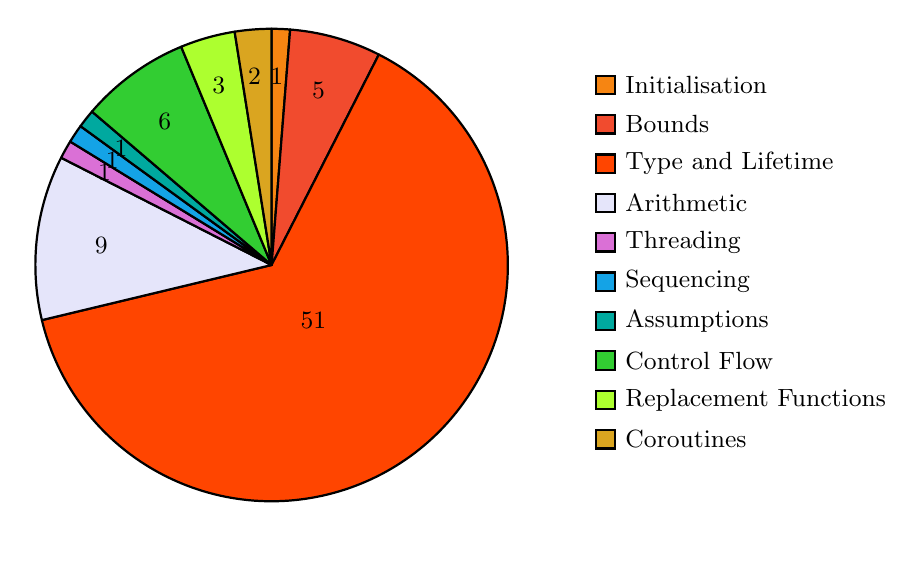
\begin{tikzpicture}
        \pie[text=legend, 
               radius=3, 
               rotate=90,
               change direction,
               color={BurntOrange, RedOrange, OrangeRed, Lavender, Orchid, Cerulean, Emerald, LimeGreen, GreenYellow, Goldenrod},
               sum=auto,
               after number = \,,   % keeps numbers tidy (adds thin space)
               /tikz/nodes={font=\small} % tweak font size if needed
            ]
            {1/Initialisation, 5/Bounds, 51/Type and Lifetime, 9/Arithmetic, 1/Threading, 1/Sequencing, 1/Assumptions, 6/Control Flow, 3/Replacement Functions, 2/Coroutines}
    \end{tikzpicture}
    \caption{Distribution of identified cases of explicit language UB across specified categories}
    \label{piechart_categories}
\end{figure}


 \renewcommand{\labelenumi}{\Roman{enumi}.}
\begin{enumerate}
\item \textbf{Initialisation} --- 1 case. Evaluating an expression that produces an indeterminate value.
\item \textbf{Bounds} --- 5 cases. Using a pointer in a way that fails to respect the range of the pointed-to object or array. Examples: incrementing a pointer beyond the past-the-end position; performing single-object delete on an operand obtained from an array-new expression;  dereferencing a pointer returned from a request for zero size.
\item \textbf{Type and Lifetime} --- 51 cases. Operations that access storage and/or use pointers or references to storage in an inappropriate way that is not already covered by Initialisation and Bounds. Examples: attempting to access a value of one type through  a pointer of a different, incompatible type; attempting to access the value of an object after its lifetime has ended. 
\item \textbf{Arithmetic} --- 9 cases. Executing an arithmetic operation whose operands fail to meet certain preconditions. Examples: division by zero; conversion of a value to a different arithmetic type that cannot represent that value. 
\item \textbf{Threading} --- 1 case. Performing two concurrent accesses, at least one of which is modifying, to the same memory location from different threads where neither access happens before the other, i.e., a data race.
\item \textbf{Sequencing} --- 1 case. Performing two concurrent accesses, at least one of which is modifying, to the same memory location from the same thread where neither access is sequenced before the other.
\item \textbf{Assumptions} --- 1 case. Reaching an \tcode{[[assume]]} declaration whose operand would not evaluate to \tcode{true}.
\item \textbf{Control Flow} --- 6 cases. Errors in control flow. Examples: flowing off the end of a function; re-entering the same declaration recursively when initialising a static variable.
\item \textbf{Replacement Functions} --- 3 cases. Executing a user-defined replacement function (\tcode{operator new}/\tcode{delete}) that fails to meet the specified requirements. Examples: returning \tcode{null} from a user-defined placement \tcode{new}; throwing an exception from a user-defined \tcode{delete}.
\item \textbf{Coroutines} --- 2 cases. Misusing coroutine machinery. Examples: destroying a coroutine that is not suspended; invoking a resumption member function for a coroutine that is not suspended.
\end{enumerate}

Figure \ref{piechart_categories} shows the distribution of the 80 identified cases of explicit core language UB across the 10 identified categories. 



The categories of Initialisation, Bounds, and Type and Lifetime correspond to the common terms \emph{initialisation safety}, \emph{bounds safety}, \emph{type safety},  and \emph{lifetime safety}, respectively, and collectively represent UB that is commonly referred to with the umbrella term \emph{memory safety}. Much of the ongoing work around how to ``make C++ safe'' is focused on these  categories (see \cite{P3081R2}, \cite{P3700R0}, and references therein).

Because unambiguously categorising a particular case of UB into either \emph{type safety} or \emph{lifetime safety} is often impossible since it concerns both, we grouped them into a single combined category, Type and Lifetime. While some cases of UB are primarily caused by type aliasing and others are primarily caused by out-of-lifetime accesses, they form a spectrum, and many common operations in C++ (e.g., using a reference) rely on \emph{both} type and lifetime constraints to be satisfied.

Remarkably, these three categories related to memory safety account for 57 cases of UB, or 71.25\% of all identified cases; the Type and Lifetime category alone accounts for 51 cases of UB, or 63.75\% of all identified cases.

The next two categories, Arithmetic and Threading, correspond to the common terms \emph{arithmetic safety} and \emph{thread safety}, respectively; the latter contains only one case of UB, data races.

The following category, Sequencing, also contains just one case of UB: unsequenced operations, such as \mbox{\tcode{i++ + ++i}}. Classifying UB due to data races and unsequenced operations into two separate categories might seem surprising at first since they have a very similar same shape (except that one is inter-thread and the other is intra-thread), but as we will see in Section~\ref{strategy}, these two categories actually require very different approaches to mitigation.

The next category, Assumptions, also contains just one case of UB: reaching an \tcode{[[assume]]} declaration whose operand would not evaluate to \tcode{true}. As we will see later, this case of UB is of a different nature than the others and warrants its own category.

The final three categories (Control Flow, Replacement Functions, and Coroutines) contain a handful of cases of UB that are less frequently discussed in the current ``safe C++'' discourse.

\subsubsection{Relevance for security}

\cite{P3656R1} asks which cases of UB are security related. The paper suggests having security experts indicate which cases of UB have security impact and use ``always'', ``never'', and ``sometimes'' tags. We are not security experts, so we do not attempt to do this here. However, we note that cases of UB commonly associated with security vulnerabilities (see, for example, the CWE list at \url{https://cwe.mitre.org/}) fall into the Initialisation, Bounds, and Type and Lifetime categories. 

Other cases of UB are not commonly exploited by malicious attackers to our knowledge. Nevertheless, some of these cases, for example those in categories Arithmetic and Threading, are a common source of program defects that do sizeable damage to existing software.

In principle, with aggressive optimising compilers any form of UB can lead to unpredictable defects and vulnerabilities. Mitigating cases of UB currently considered to be the most critical security concern will simply remove the easiest routes of attack from the table, and any UB not yet addressed may become the new major candidate for attackers to leverage for nefarious purposes.  Therefore, prioritising implementation based on current trends amongst malicious actors, though helpful, should not be used to limit the scope of our work on improving the C++ language specification (see \cite{Sutter2024}, \cite{P3500R1}, and \cite{P3578R0}).

\subsection{Diagnosability} 
\label{diagnose}

The second question \cite{P3656R1} asks is which cases of UB are ``efficiently locally diagnosable''. In this paper, we split this question into three separate questions: whether diagnosis can happen statically or whether it needs to happen dynamically (i.e., at runtime), whether such diagnosis can be performed locally, and the run-time cost of such diagnosis (whether performed locally or not).

\subsubsection{Static vs. dynamic diagnosis}
\label{statically}

A commonly asked question is ``why does the committee not simply make all the UB ill-formed instead''? The answer is that in order for that to happen, it would be necessary to determine statically --- i.e., at compile time --- whether a given operation in a C++ program would lead to UB when executed at runtime. However, whether a C++ program will have UB when executed is fundamentally a \emph{runtime} property, i.e., the answer depends on run-time values unknown at compile time (for example, the run-time value of a pointer or an integer). Therefore, in the vast majority of cases, such a compile-time determination cannot be made. In fact, in our entire list of 80 cases of UB, we cannot identify \emph{any} cases that can unconditionally be diagnosed at compile time.

Of course, static analysis is still useful and widely used in the field. There are many situations where static analysis \emph{can} detect a bug that would lead to UB when executed, because the relevant values or conditions happen to be known at compile time in the particular program at hand. However, given an existing C++ program, any approach based on static analysis fundamentally has to choose between \emph{false positives} (rejecting code for which no proof can be constructed one way or another, even if that code happens to be correct) and \emph{false negatives} (accepting incorrect code that will lead to UB when executed). 

Crucially, whether a pointer or reference refers to a valid object of the correct type within its lifetime at a given point in time (``memory safety''), the relevant property for addressing UB in the Initialisation, Bounds, and Type and Lifetime categories, seems to be fundamentally unprovable at compile time in the general case (see \cite{Baxter2024}).

As we will see in Section~\ref{strategy}, despite these fundamental limitations there are things we can (and should) do in the C++ Standard to enable static analysis to construct a proof in more cases, such as adding annotations (\ref{annotations}), subsetting the language (\ref{subsetting}), and providing replacement features (\ref{newfeatures}). However, for existing C++ programs, reliably detecting cases of UB without rejecting correct code will inevitably have to leverage \emph{run-time} detection, i.e., the insertion of additional run-time checks when compiling the program. We therefore focus on such run-time detection for the remainder of this analysis.

\subsubsection{Locality of diagnosis}
\label{locally}

An important property for diagnosis of UB is whether such diagnosis (whether static or dynamic) can be performed \emph{locally}, i.e. without keeping track of additional information across the entire program that is not available within the C++ abstract machine (achievable with additional instrumentation of the kind that is implemented in sanitisers, such as ASan and UBSan) and without analysing code in other branches (which is limited by the Halting problem) or on the other side of a function call boundary (which might be located in another TU and therefore inaccessible).

Most cases of UB in the Initialisation, Bounds, and Type and Lifetime categories are, in general, \emph{not} locally diagnosable. They could potentially be made locally diagnosable in the future with the introduction of novel features such as lifetime annotations \cite{P2771R1} or ``ghost data'' \cite{Lippincott2025} which are the subject of ongoing research. We discuss some of these approaches in Section~\ref{strategy}; here, we focus on the status quo in  Standard C++.

In the Bounds category, 
\{expr.add.out.of.bounds\} 
and \{expr.add.sub.diff.pointers\} 
are partially locally diagnosable (only if the array bound is statically known). In the Type and Lifetime category,
\{expr.static.cast.downcast.wrong.derived.type\},
\{expr.unary.dereference\}, 
\{conv.ptr.virtual.base\}, and
\{expr.dynamic.cast.lifetime\}
are partially locally diagnosable (for the null pointer case).
\{expr.mptr.oper.member.func.null\} is locally diagnosable because this case requires \emph{only} a null pointer check.
\{basic.align.object.alignment\} is locally diagnosable by checking the alignment of storage when creating an object at run time.
\{expr.assign.overlap\} is locally diagnosable by checking the overlap of the two address ranges. (The ranges are known because the address and \tcode{sizeof} are known at run time for both the source and the destination object.) \{class.abstract.pure.virtual\} is locally diagnosable by adding a run-time check to  the pure virtual function stub to which the base class vtable points. None of the other cases of UB in the Initialisation, Bounds, and Type and Lifetime categories are locally diagnosable.

All cases of UB in the Arithmetic category are locally diagnosable since they are all cases of an arithmetic operation producing a value that is somehow inappropriate (mathematically invalid, not representable in the target type, etc.) and that value can be inspected at run time.

UB in the Threading category (\{intro.races.data\}) is not locally diagnosable, but UB in the Sequencing category (\{intro.execution.unsequenced.modification\}) is. 

UB in the Assumption category (\{dcl.attr.assume.false\}) is, in principle, locally diagnosable by evaluating the operand of the assumption and verifying that the resulting value, contextually converted to \tcode{bool}, equals \tcode{true}. However, if that evaluation has any side effects, such a check could alter the observable state of the program. Therefore, even if the given assumption holds and no UB occurs, the check itself might render the program invalid by altering its state. Thus, this case of UB is  meaningfully diagnosable in any automated fashion only if the operand has no side effects when evaluated. However, proving that the operand has no side effects is generally impossible to do efficiently and is outright impossible in the presence of an opaque function call.

Some cases of UB in the Control Flow category are locally diagnosable. \{stmt.return.flow.off\} and \{stmt.return.coroutine.flow.off\} can be diagnosed by inserting a check at the end of every function body that does not end with a \tcode{return} or \tcode{co_return} statement. \{dcl.attr.noreturn.eventually.returns\} can be diagnosed by inserting a check into every function declared \tcode{[[noreturn]]}.

Some cases of UB in the Replacement Function category are partially or fully locally diagnosable. In particular, some of the constraints specified in \{basic.stc.alloc.dealloc.constraint\} and \{expr.new.non.allocating.null\} are locally diagnosable, while others are not. In particular, we can check locally that a deallocation function does not exit via an exception and that an allocation function does not return null. However, checking the other constraints (locally or at all) is generally not possible.

Finally, all cases of UB in the Coroutine category are not locally diagnosable since being so would require tracking run-time state information that is not currently maintained within the coroutine handle in most implementations.

Overall, as shown in Figure~\ref{piechart_locally}, only 18 cases of UB (22.5\% of all cases) are unconditionally locally diagnosable at runtime, while 58 cases of UB (72.5\%) are not; these cases require instrumentation of the code in order to be diagnosed at runtime. We will discuss these requirements in more detail in Section~\ref{cost_nonlocal}.

%~~~~~~~~~~~~~~~~~~~~~~~~~~~~~~~~~~~~~~~~~~~~~~~~~~~~~~~~~~~~~~~~~~~
\vspace{5mm} % added manually to create enough space between text and piechart
\begin{figure}[t!]
    \centering
    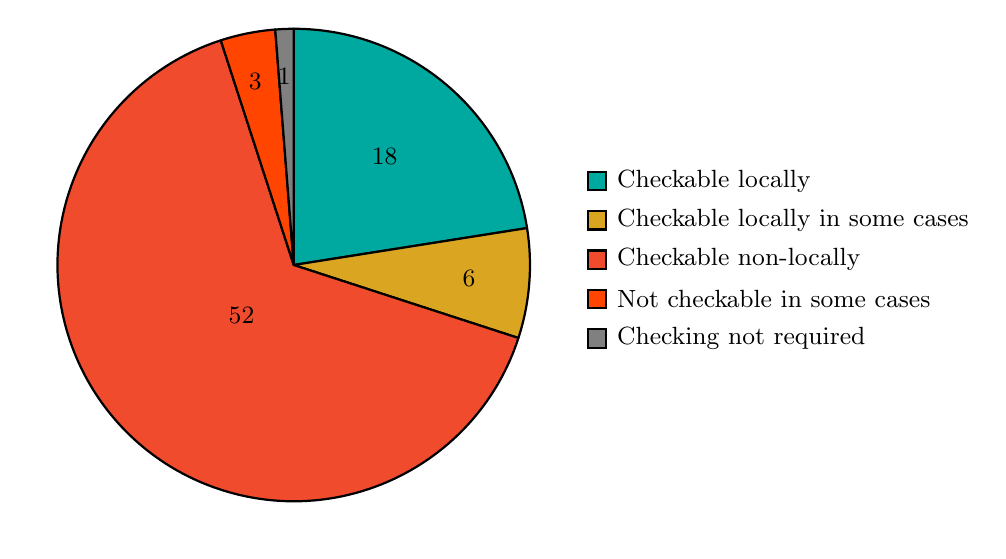
\begin{tikzpicture}
        \pie[text=legend, 
               radius=3, 
               rotate=90,
               change direction,
               color={Emerald, Goldenrod, RedOrange, OrangeRed, Gray},
               sum=auto,
               after number = \,,   % keeps numbers tidy (adds thin space)
               /tikz/nodes={font=\small} % tweak font size if needed
            ]
            {18/Checkable locally, 6/Checkable locally in some cases, 52/Checkable non-locally, 3/Not checkable in some cases, 1/Checking not required}
    \end{tikzpicture}
    \caption{Runtime diagnosability of explicit core language UB}
    \label{piechart_locally}
\end{figure}
%~~~~~~~~~~~~~~~~~~~~~~~~~~~~~~~~~~~~~~~~~~~~~~~~~~~~~~~~~~~~~~~~~~~

\subsubsection{Cost of local diagnosis}
\label{cost_local}

Considering locally checkable cases of UB separately from non-locally checkable ones is useful to estimate the cost of diagnosis. For locally diagnosable cases, some kind of run-time check --- an \emph{assertion} --- could be inserted by the implementation and then evaluated at run time. The total cost of diagnosis is, therefore, equal to the cost of evaluating that check multiplied by the number of times the check needs to be evaluated.

Note that in this paper, we study the theoretical, relative cost based on the current specification of the C++ language. We do not, however, measure the actual cost in existing tooling that implements such checks, nor do we present benchmarks in this paper; such studies are left for future work.

That said, the cheapest kind of check --- and the only one that has (almost) no overhead for the happy path --- is the ``fail if you get here'' check, equivalent to a \tcode{pre}/\tcode{post}/\tcode{contract_assert(false)}. This kind of check is sufficient to diagnose \{class.abstract.pure.virtual\}, \{stmt.return.flow.off\}, \{stmt.return.coroutine.flow.off\}, and \{dcl.attr.noreturn.eventually.returns\}.

A slightly more expensive but still cheap and optimiser-friendly kind of check is a null check, required to diagnose the null pointer cases  
(\{expr.static.cast.downcast.wrong.derived.type\},
\{expr.unary.deref\-erence\},
\{conv.ptr.virtual.base\},
\{expr.dynamic.cast.lifetime\}, 
\{expr.mptr.oper.member.\linebreak[3]func.null\}, and
\{expr.new.non.allocating.null\})
as well as division by zero (\{expr.mul.div.by.zero\}).

Integer comparisons are similarly cheap and optimiser-friendly and are   required for bounds checks with statically known array bounds
(\{expr.add.out.of.bounds\} and
\{expr.add.sub.diff.pointers\})
as well as for \{expr.shift.neg.and.width\} 
and \{intro.execution.unsequenced.modification\}.

Beyond this, a number of UB cases can still be checked by a straightforward arithmetic expression but with increasingly expensive expressions: \{expr.assign.overlap\} requires computing whether two integer ranges overlap, and  \{basic.align.object.alignment\} requires computing an integer modulo. 

At the expensive end of the locally diagnosable UB spectrum are run-time checks for which there is no corresponding C++ expression; instead, the compiler would have to generate more complex ``magic'' checks based on knowledge unavailable in the C++ abstract machine. In particular, this case applies to all arithmetic UB except \{expr.add.out.of.bounds\} and
\{expr.add.sub.diff.pointers\}. The compiler would have to validate the bit patterns of values of arithmetic types according to knowledge it has about how values of such types are represented on the targeted platform. Such checks can be done locally, but they can slow operations involving built-in types and, in particular, floating-point types.

In addition to the cost of the check itself, we need to consider the frequency with which these checks would need to be done. Checks that would need to happen once when a function is called or when a function returns are likely to be acceptable in most scenarios. Extensive checks for arithmetic UB will probably be acceptable in fewer scenarios because such checks have the potential to significantly slow arithmetic operations, which are performance sensitive in many contexts. On the extreme end, if we wanted to diagnose \{intro.execution.unsequenced.modification\} via a run-time check, the check itself would be fairly inexpensive, but the compiler would have to identify all potential read operations that are not sequenced with respect to each given write operation and then insert checks to identify if those operations are actually going to reference the same address.

\subsubsection{Cost of non-local diagnosis}
\label{cost_nonlocal}

For UB that is not locally diagnosable (which is most of the UB in C++), we need to consider the cost of the required additional instrumentation. To get an idea of that cost, we must nail down exactly which additional properties that are not normally known from within the C++ abstract machine would need to be tracked by such instrumentation. This tracking would need to happen at run time throughout the \emph{entire} program; checks relying on the tracked information would have to be inserted for \emph{every} run-time operation that may be affected by such UB.
The full list is available in \hyperref[appendix]{Appendix~A}, and we provide an overview below.

To diagnose \emph{all} cases of UB in the memory safety categories of Initialization, Bounds, and Type and Lifetime, instrumentation would have to track all the following properties:

\begin{itemize}
\item Provenance of all pointers and pointers-to-member
\item For all storage, whether it has been allocated or freed
\item For all storage, whether it has been initialised
\item For all storage, whether it has been created such that it can hold implicit lifetime objects
\item For all storage, the type of the object associated with it (if any), including whether it is \tcode{const} or \tcode{volatile}
\item For all objects, whether their lifetime has been started or ended
\item For all objects, whether they are currently being constructed or destroyed
\item The dynamic type of all \emph{non}-polymorphic objects of class type
\item For all references, whether they have been initialized
\item For all addresses that point to  functions, the type of the function
\end{itemize}

To diagnose UB in the Threading category, instrumentation would have to track, for \emph{all} memory accesses, from which threads that memory is accessed and when these accesses synchronise with each other. Doing this exhaustively is not practically possible; however, instrumentation that is capable of diagnosing a subset of cases exists in the form of sanitisers (TSan).

The non-locally-diagnosable UB in the Control Flow category concerns operations that are not allowed during construction and destruction of objects with static or thread-local storage duration (\{basic.start.main.exit.during.destruction\} and \{basic.start.term.use.after.destruction\}). To diagnose these, instrumentation would have to insert guards tracking whether such objects are currently being constructed and destroyed.  

Finally, to diagnose UB in the Coroutine category, instrumentation would have to track the suspension state associated with every coroutine handle.

As we know from existing sanitisers, such instrumentation is expensive enough that it is almost never affordable in production. If we were to add instrumentation covering \emph{all} of the above, we would remove vast swathes of UB from the language, but performance would worsen by an order of magnitude, unless special hardware-acceleration or some other radically new technology for these checks becomes available. We discuss some of the consequences of this fundamental dilemma in Section~\ref{strategy}.

Given the substantial overhead of such instrumentation in both run-time cost and additional memory consumption, the cost of the actual checks themselves (whether a specific pointer is valid at a specific time, etc.) is not particularly important for non-local diagnosis because the performance penalty would be dominated by the instrumentation overhead.

\subsection{Existence of well-defined replacement behaviour}
\label{replacement}


For existing code that cannot be modified in-source, removing run-time UB from the C++ language is essentially equivalent to changing the specification of operations that can have run-time UB to have some form of well-defined behaviour instead. A useful question is therefore: for which cases of UB is it possible to specify such well-defined \emph{replacement behaviour}?

For the purposes of this analysis, we need to be careful with delineating what exactly we mean by replacement behaviour. If it is possible to insert a run-time check guarding a particular case of UB (e.g., a bounds check, a null pointer check), we can specify well-defined behaviour for the case when this check fails (e.g., terminate the program, throw an exception) which guarantees that we never actually execute the operation that would have run-time UB, thus avoiding it. However, regardless of the existence of that check, there are also cases where we can give well-defined behaviour to the operation itself, such that continuing to evaluate that operation does not lead to run-time UB even in the case where there is a bug that would cause UB with the current language specification. This is precisely what we mean by giving an operation replacement behaviour.

As we will discuss in more detail in Section~\ref{strategy}, we can conceptually distinguish between two types of replacement behaviour --- \emph{refined} and \emph{erroneous} behaviour --- depending on whether the replacement behaviour is considered correct or incorrect (despite no longer being undefined). In any case, for either type of replacement behaviour to actually happen, the compiler must be able to lay down the necessary instructions at compile time. Simultaneously, as discussed in Section~\ref{statically}, in the vast majority of cases core language UB is fundamentally \emph{not} diagnosable at compile time, as whether or not the UB will occur depends on run-time parameters. Replacement behaviour can therefore not depend on knowing that an error occurred. For non-locally-diagnosable UB, replacement behaviour also cannot depend on any additional instrumentation being present.




For this paper, we systematically identified all cases of core language UB for which either form of replacement behaviour can be meaningfully defined. This section gives an overview; the full list can be found in \hyperref[appendix]{Appendix~A}. As we will see, for most cases of UB, replacement behaviour does not exist, and if it does, it is often not cheap.

For UB in the Initialization category (\{basic.indet.value\}), replacement behaviour is sometimes possible for built-in types: an operation that would currently return an indeterminate value can be specified to return \emph{some} value instead.


We could consider returning a specific value such as 0, or returning some unspecified value (as a form of refined behaviour). However, doing so removes the ability for tools to recognise that a program defect is present (see \cite{P2754R0}). The most meaningful option is to make it return an erroneous value (a form of erroneous behaviour). For variables with automatic storage duration, this replacement behaviour is already part of C++26 as EB via \cite{P2795R5} because for this case, the replacement behaviour is particularly cheap. The same  behaviour could also be employed for dynamically allocated variables but at greater cost (see \cite{P2723R1} Section 6 for discussion).

On the other hand, producing an erroneous value (instead of, for example, the value that happened to be in memory where an object was incorrectly presumed to have been initialised) requires having a point in time where a fallback value can be unconditionally placed in memory, such as when passing the declaration of an automatic variable; there are cases where such a point cannot be determined.

Further, we cannot in general define replacement behaviour for uninitialised variables of user-defined type. Even if we could zero out all the underlying storage for user-defined types (or overwrite it with some other known bit pattern), doing so does not always produce, for that type, a valid value that can be accessed without UB. (Consider a user-defined type that relies on a member pointer always being dereferenceable.) Therefore, \{basic.indet.value\} does not have replacement behaviour for the general case.



Practically \emph{none} of the UB in the categories of Bounds and Type and Lifetime have any plausible replacement behaviour. The only exception is \{conv.lval.valid.representation\}: if the bits in the value representation of an object of built-in type are not valid for that type, the compiler could instead coerce the value into an erroneous value.\footnote{This property of \{conv.lval.valid.representation\} is a potential argument for placing this case of UB into the Arithmetic category instead of the Type and Lifetime category as we did here.} For example, in the code example given in the C++ working paper,



\begin{codeblock}
bool f() {
  bool b = true;
  char c = 42;
  memcpy(&b, &c, 1);
  return b;         // undefined behavior if \tcode{42} is not a valid value representation for \tcode{bool}
}
\end{codeblock}



the UB could be replaced by well-defined behaviour by appropriately bit-masking every accessed \tcode{bool} value (and considering the result erroneous if the bit-mask operation changed the value). Similar mitigations could be put in place for other built-in types since the space of allowed bit representations for values of those types, for the targeted platform, are known to the compiler. The caveat is that such mitigations would potentially incur a significant performance overhead on many simple operations that involve built-in types.

All UB in the Arithmetic category has the same possible replacement behaviour: if an arithmetic operation would produce an inappropriate value, it can be coerced into some other value instead. We could contemplate refined behaviour in the form of a concrete value (e.g., saturate or wraparound for signed integer overflow, choose the closest valid value for invalid conversions) or erroneous behaviour in the form of an erroneous value being produced. In either case, such replacement behaviour will incur significant performance overhead on common arithmetic operations.

Defining replacement behaviour for UB in the Threading category (\{intro.races.data\}) is in principle possible: we could make all primitive memory accesses implicitly atomic, as in the Java memory model. The overhead incurred by such a model will heavily depend on the memory model of the underlying hardware; on weakly-ordered platforms, such as ARM,
it will be larger than on strongly-ordered platforms such as x86. Note that while such replacement behaviour is well-defined, it still fails to prevent many real bugs that result from incorrect application of concurrency since user-defined types with multiple members can still be easily observed with inconsistent (``torn'') states if no proper synchronisation is performed.


The replacement behaviour for UB in the Sequencing category (\{intro.execution.unsequenced.modifica\-tion\}) is much more straightforward: we can define that the unsequenced operations happen in some unspecified order. This behaviour can still have performance overhead in the form of losing  optimisation opportunities, but such overhead will likely be manageable. 


The replacement behaviour for UB in the Assumption category (\{dcl.attr.assume.false\}) is trivial: just ignore the assumption, instead of optimising based on it. The performance overhead is limited to losing any optimisation opportunities from placing the assumption there. Of course, this mitigation makes the assumption itself completely useless. We will discuss this case in more detail in Section~\ref{assume}.

Finally, we can define partial replacement behaviour for two cases of UB in the Control Flow category  (\{stmt.return.flow.off\} and \{stmt.return.coroutine.flow.off\}): when the function or coroutine would return a value of built-in type, we can define that flowing off the end returns an erroneous value. This case is analogous to \{basic.indet.value\}; again, no plausible replacement behaviour exists for user-defined return types in the general case.

Overall, as shown in Figure~\ref{piechart_replacement}, we can define meaningful replacement behaviour for only 16 cases of UB (20\% of all cases). In addition, in 3 cases, this is only possible when the operation in question produces a value of built-in type. Unconditional replacement behaviour exists for only 13 cases of UB (16.25\% of all cases). In all of these cases, the replacement behaviour consists of erroneous behaviour; in most cases, removing the UB in this manner introduces significant runtime cost.


%~~~~~~~~~~~~~~~~~~~~~~~~~~~~~~~~~~~~~~~~~~~~~~~~~~~~~~~~~~~~~~~~~~~
\vspace{5mm} % added manually to create enough space between text and piechart
\begin{figure}[t!]
    \centering
    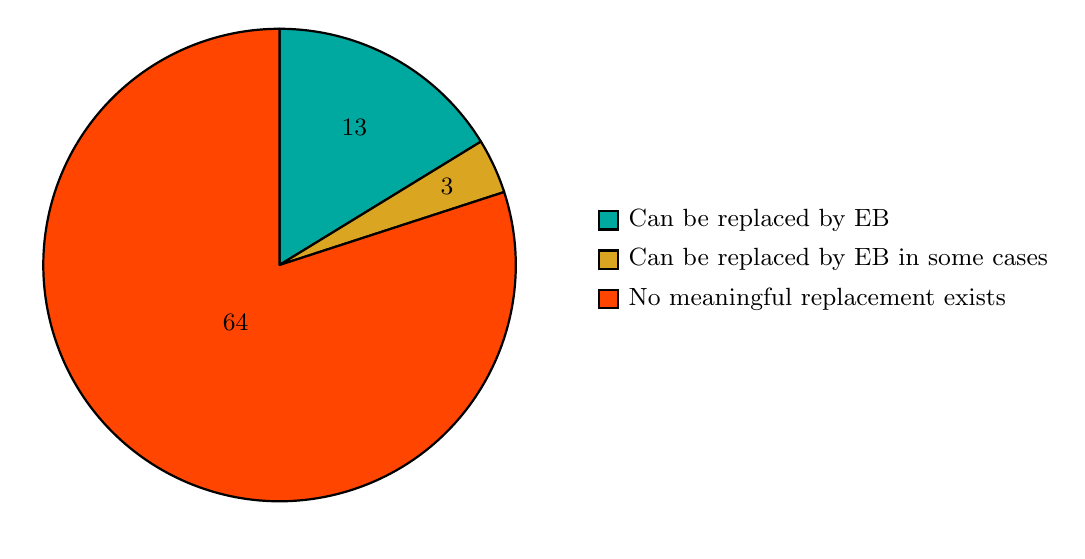
\begin{tikzpicture}
        \pie[text=legend, 
               radius=3, 
               rotate=90,
               change direction,
               color={Emerald, Goldenrod, OrangeRed, Gray},
               sum=auto,
               after number = \,,   % keeps numbers tidy (adds thin space)
               /tikz/nodes={font=\small} % tweak font size if needed
            ]
            {13/Can be replaced by EB, 3/Can be replaced by EB in some cases, 64/No meaningful replacement exists}
    \end{tikzpicture}
    \caption{Existence of well-defined replacement behaviour for explicit core language UB}
    \label{piechart_replacement}
\end{figure}
%~~~~~~~~~~~~~~~~~~~~~~~~~~~~~~~~~~~~~~~~~~~~~~~~~~~~~~~~~~~~~~~~~~~


\section{Strategy}
\label{strategy}

Having performed an in-depth analysis of all explicit core language UB in the C++ working paper in Section~\ref{analysis}, we can use the results of this analysis to develop a holistic strategy for systematically detecting, mitigating, and ultimately removing UB across the entire C++ programming language specification. Our goal is for this strategy to guide the development of the core language UB white paper \cite{P3656R1} as well as future versions of Standard C++.

The outline of this strategy is illustrated in Figure~\ref{fig_magicslide}, an updated version of the diagram on slide 53 in \cite{P3754R0} (a.k.a. the ``magic slide'') that we presented to EWG in Sofia and that EWG approved as a basis for the core language UB white paper.


%~~~~~~~~~~~~~~~~~~~~~~~~~~~~~~~~~~~~~~~~~~~~~~~~~~~~~~~~~~~~~~~~~~~
\vspace{3mm}
\begin{figure}[h]
\begin{center}
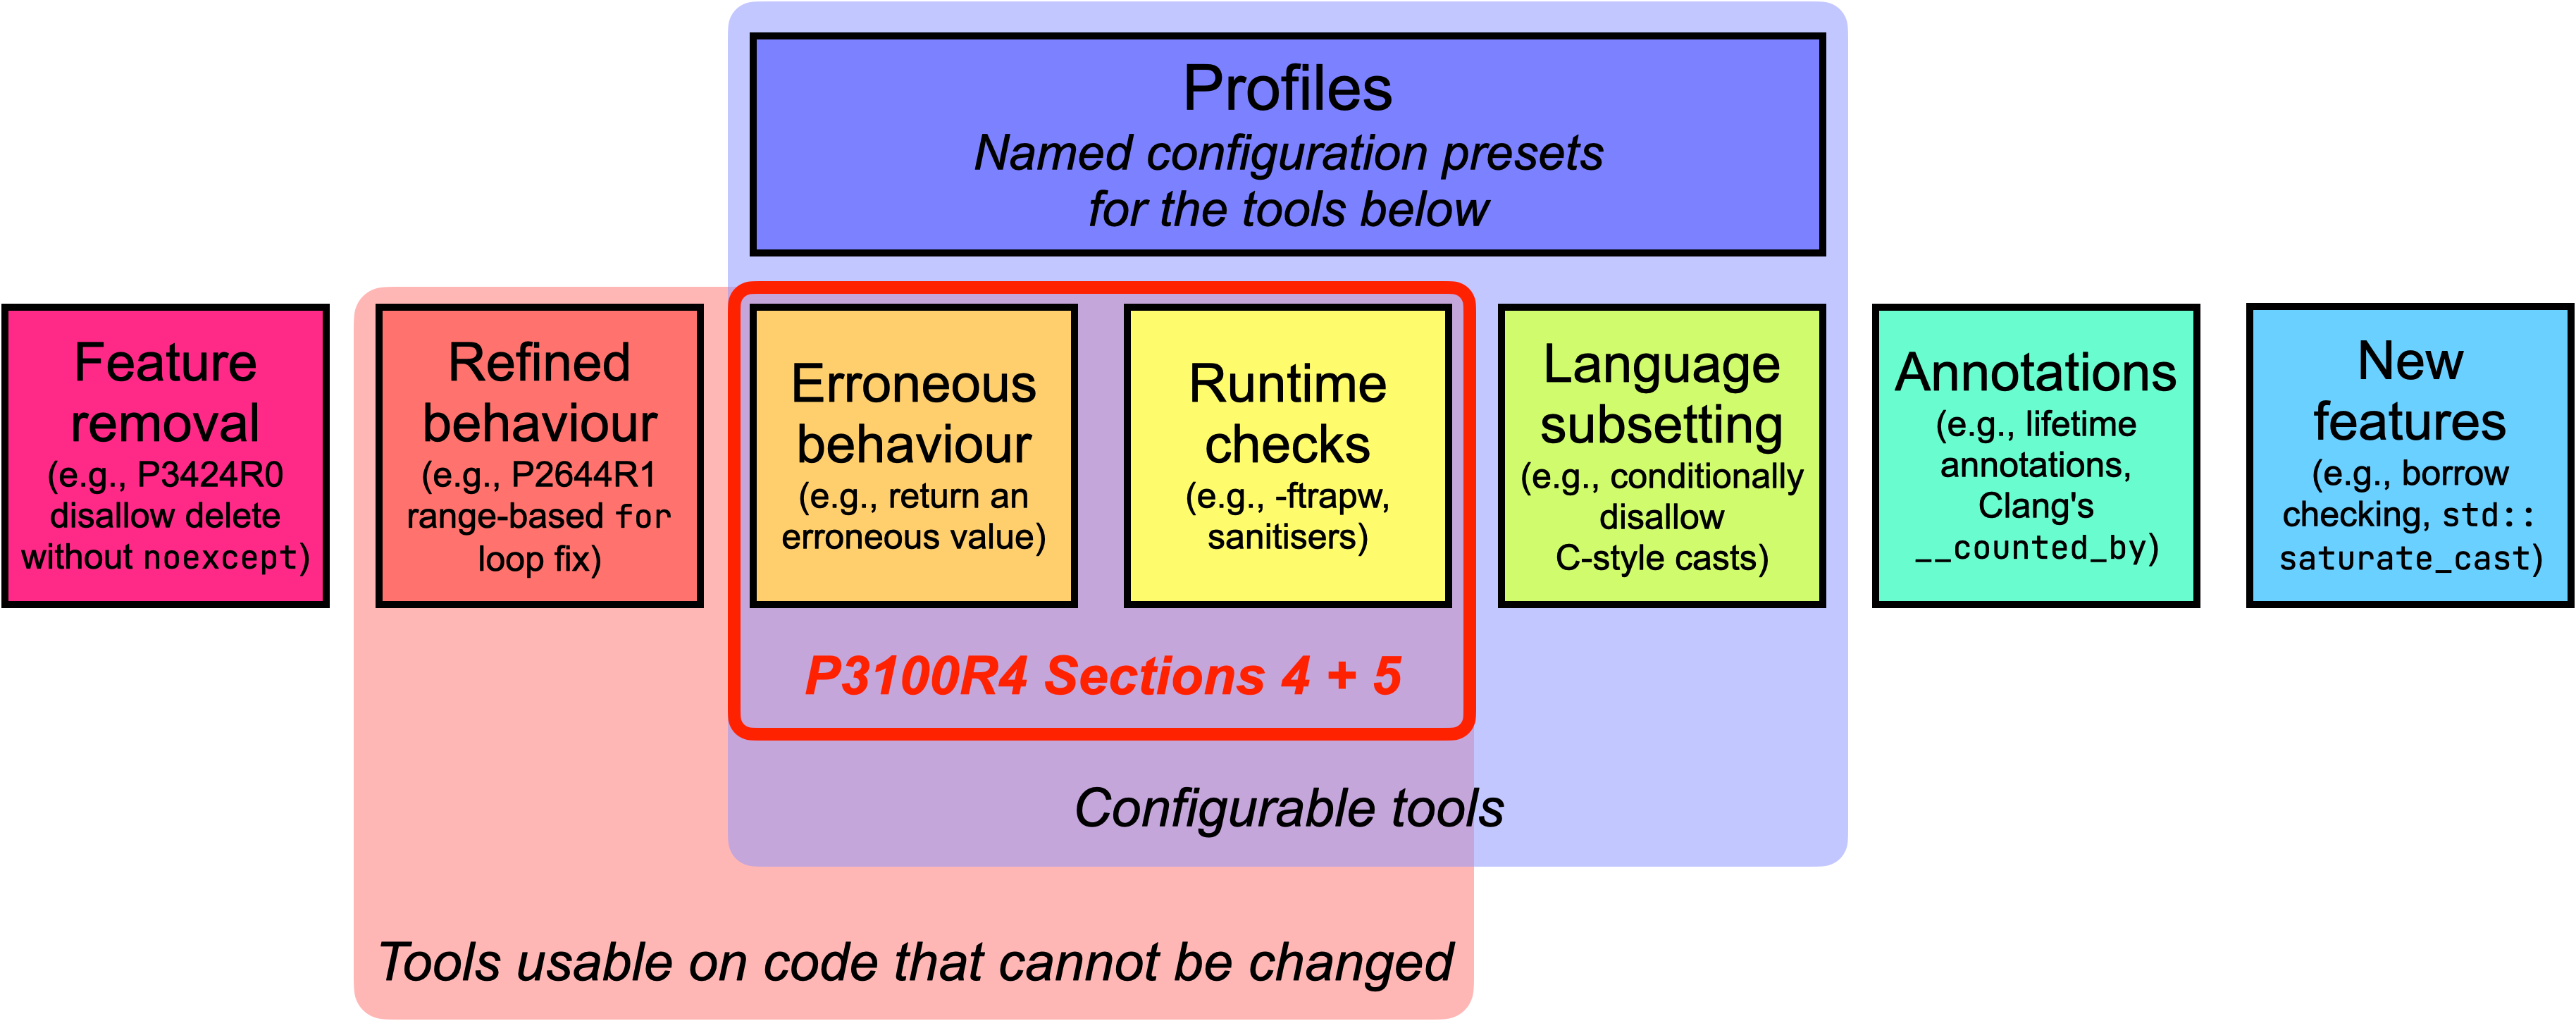
\includegraphics[scale=0.256]{images/p3100_magicslide.png}
\end{center}
\caption{Overview of the proposed holistic strategy for removing UB from the C++ language: seven orthogonal tools plus Profiles as a higher-level feature specified on top of these tools. The red rectangle in the centre illustrates the scope of the proposal in Sections~\ref{design} and \ref{wording} of this paper.}
\label{fig_magicslide}
\end{figure}
%~~~~~~~~~~~~~~~~~~~~~~~~~~~~~~~~~~~~~~~~~~~~~~~~~~~~~~~~~~~~~~~~~~~

\subsection{Overview}

The proposed strategy is composed of seven basic tools that are orthogonal to each other: refined behaviour, erroneous behaviour, insertion of run-time checks, feature removal, language subsetting, the introduction of annotations, and the introduction of entirely new language features. In section~\ref{tools}, we describe each tool and discuss which cases of UB identified in this paper it can be applied to.

Three of these tools (refined behaviour, erroneous behaviour, and run-time checks) have the interesting property that they are usable without any source changes and can thus be used to remove UB from existing legacy C++ programs whose source code cannot be changed for whatever reason.

Further, in order to be usable effectively in practice, three of these tools (erroneous behaviour, run-time checks, and language subsetting) need to be configurable by the user, either via compiler options or directly in source. This design space is discussed in more detail in Section~\ref{config}.

Finally, several of the available tools overlap in scope with \emph{Profiles}, another proposed feature currently in development. A discussion of how Profiles fit into our proposed strategy can be found in Section~\ref{profiles}.

\subsection{Scope}

Our proposed strategy for removal of explicit core language UB focuses on tools that can be portably specified within the C++ Abstract Machine. We therefore do not consider, in this paper, efforts that operate largely outside of the C++ Abstract Machine framework. One noteworthy effort that falls into the latter category is  \cite{P3627R0}, which proposes a profile for preventing remote code execution (RCE) by employing implementation-defined techniques such as stack isolation and address space layout randomisation (ASLR).

Further, as discussed in \cite{P3700R0}, making C++ ``safe''\footnote{In this paper, we avoid unqualified uses of the terms ``safe'' and ``safety'' because of their ambiguity. As discussed in \cite{P3376R0}, \cite{P3500R1}, and \cite{P3578R0}, it is critically important to distinguish between conflicting usages of those terms, such as functional safety, language safety, memory safety, etc.} consists of more than mitigating explicit core language UB. We already touched upon implicit UB and language UB in Section~\ref{enum_scope}. Beyond those, there are many other classes of bugs unrelated to UB that can compromise the functional safety, security, and correctness of a C++ program. Such bugs include resource leaks, termination errors, and logic errors. 

While there are tools available to address these classes of bugs (for example, logic errors can often be avoided by using strongly typed utilities such as \cite{P3045R6}), and there is interesting ongoing work in those areas, they are out of scope for the strategy proposed here. At least for now, we explicitly target the core language UB white paper \cite{P3656R1} and therefore limit the scope of the strategy described here to explicit core language UB. 

\subsection{Tools}
\label{tools}

\subsubsection{Feature removal}
\label{removal}

The first and most blunt tool in our toolbox is to make a C++ operation that would otherwise lead to run-time UB unconditionally ill-formed, i.e., to remove it from the language --- either immediately or via a deprecate-remove cycle spanning multiple releases of the C++ Standard.

However, we generally do not consider it acceptable to break an existing, \emph{correct} program by using this tool (or any of the other proposed tools). If we want to strictly follow this principle, usage of the removal tool would have to be restricted to cases where we can determine at compile time that the given operation will definitely have UB when executed.\footnote{One could argue that even then, the program is not necessarily incorrect unless that operation actually ends up being executed during runtime. This is not something a C++ compiler can reason about unless the operation in question is either lexically inside \tcode{main} or is provably being called from \tcode{main}.} As discussed above in Section~\ref{statically}, there is not a single case of UB in our list where such a determination can generally be made.

A slightly more aggressive approach would be to unconditionally remove a feature if we can determine at compile time that it always \emph{either} exhibits UB \emph{or} does nothing useful. This approach is being proposed in \cite{P3424R0} for the case of having a deallocation function (i.e., a user-defined \tcode{delete} operator) that is not declared \tcode{noexcept}. Since exiting a deallocation function via an exception is UB, a deallocation function that is not declared \tcode{noexcept} either exhibits UB (if an exception ends up being thrown from it) or does nothing useful (if no such exception is ever being thrown). Therefore, the paper proposes to deprecate deallocation functions with an explicit non-throwing \emph{noexcept-specifier} and making deallocation functions with a potentially-throwing \emph{noexcept-specifier} ill-formed.

We are currently not aware of any other areas in the C++ Standard where this tool could be successfully applied, but it is worth keeping it in our toolbox in case such areas will be discovered in the future.

\subsubsection{Refined behaviour}
\label{refined}

Some cases of UB can be addressed by unconditionally changing their runtime semantics to some well-defined behaviour. We have extensively used this option in the past to gradually remove UB from the language; examples of successfully applying this tool in the C++ Standard are the introduction of implicit lifetime types in C++20 \cite{P0593R6} which gave defined behaviour to certain situations when a pointer to raw allocated memory is being cast to a pointer of object type, as well as the range-based for loop fix in C++23 \cite{P2644R1},  which extended the lifetime of certain temporary objects across the duration of executing the loop, thus avoiding UB due to dangling references. 

We expect that in the C++ Standard there will be relatively few remaining situations where this tool can be used effectively. For the vast majority of UB that remains in C++ today, unconditionally refining the behaviour is either not possible with any sensible semantics or would lead to unacceptable performance degradations. Moreover, in many cases where replacement behaviour is possible, unconditionally refining the behaviour would effectively mask the bug and make it impossible for tools to distinguish it from correct usage. It is therefore preferable to replace the behaviour with erroneous behaviour instead (see next section). 

\subsubsection{Erroneous behaviour}
\label{erroneous}

Some cases of UB can be addressed by replacing it with well-defined replacement behaviour, but specifying that replacement behaviour as \emph{erroneous}, that is, well-defined but considered incorrect. The purpose of introducing erroneous behaviour is to not remove the bug, and to leave tools with the possibility of diagnosing it, but at the same time to place a limit on the program behaviour in the face of the bug and in particular to prevent the bug from creating a security vulnerability.

We introduced the concept of erroneous behaviour in C++26 and added one instance of it: producing an erroneous value (instead of exhibiting undefined behaviour) when reading a default-initialised automatic variable of arithmetic type \cite{P2795R5}. In addition, erroneous behaviour for missing return from assignment is currently being proposed in \cite{P2973R0}.

\cite{P2795R5} already contains a section with a preliminary list of other cases of UB which could be replaced with erroneous behaviour. In this paper, we improve upon that preliminary list by providing a concrete list in \hyperref[appendix]{Appendix~A}. For all cases identified in Section~\ref{replacement} as having well-defined replacement behaviour (13 cases unconditionally plus 3 cases for built-in types only), we propose to introduce that behaviour as erroneous. In Sections~\ref{design} and \ref{wording} of this paper, we provide a concrete specification for how to perform the necessary replacement in the C++ Standard.

\subsubsection{Run-time checks}
\label{checks}

As we saw in Section~\ref{diagnose}, the large majority of UB (76 cases out of 80) can in principle be diagnosed by inserting and performing a suitable runtime check. The check verifies the conditions necessary for the operation in question to have well-defined behaviour at runtime. It also acts as a guard against the UB: if the check fails, the program can be terminated, thus preventing the undefined behaviour from occurring.

While such runtime checks invariably add runtime overhead, they are very effective at both diagnosing bugs and removing security vulnerabilities. In Sections~\ref{design} and \ref{wording} of this paper, we propose a generic framework for systematically adding runtime checks to C++ core language constructs via implicit contract assertions.

Implicitly generated runtime checks are widely deployed in the field today. Checks that can be generated locally by the compiler are often provided via compiler flags, for example the \tcode{-ftrapv} flag in GCC that checks for signed integer overflow and terminates the program on failure. Checks that require additional instrumentation to perform are provided by various flavours of sanitisers such as ASan, UBSan, etc.

\subsubsection{Language subsetting}
\label{subsetting}

While practically no C++ operation can, in the general case, be proven at compile time to exhibit UB at runtime, there are a number of operations that are particularly prone to exhibiting UB at runtime when not used correctly; such operations are colloquially known as ``unsafe''. Examples of such operations are C-style casts (which can silently fall back to \tcode{reinterpret_cast}) and pointer arithmetics. Compilers and linters already provide options to statically flag the usage of such features as a potential source of bugs. We could go one step further and make such constructs ill-formed, particularly if there are ``safer'' alternative features that provide equivalent functionality. 

However, in such cases, we cannot make these constructs \emph{unconditionally} ill-formed, as this would break a significant number of correct C++ programs deployed in the field. Therefore, we need to use a tool different from simple removal (Section~\ref{removal}). The required tool is called \emph{language subsetting}: specifying named \emph{subsets} of the C++ language that do not contain the ``unsafe'' features and that the user can opt into. This tool can be very useful for codebases that can be modernised or are being newly written.

While we do not propose a concrete specification for language subsetting in this paper, such a specification is being developed in \cite{P3716R0}. A number of principles need to be considered for designing this tool correctly: subsetting the language should never be allowed to alter the semantics of well-formed code, subsets must always combine orthogonally, and so forth. 

\subsubsection{Annotations}
\label{annotations}

Some cases of UB can be mitigated by language-level annotations that provide additional information that can be propagated across the interface boundaries of a C++ program. Such information can turn cases of UB that are \emph{not} locally diagnosable (which is the majority of UB today, see Section~\ref{diagnose}) into cases that \emph{are} locally diagnosable.

An example of a standard proposal in this area are the lifetime annotations proposed in \cite{P2771R1}. An example of such annotations deployed in the field as non-standard vendor extensions is the \tcode{__counted_by} attribute introduced in Clang 18. This attribute allows the user to propagate information about array bounds to enable automatic out-of-bounds checks. Such attributes are a great example for how different tools that form the proposed strategy, while being usable independently from each other, can also work together to help each other cover even more cases of UB.

\subsubsection{New features}
\label{newfeatures}

Finally, some cases of UB can be addressed by providing entirely new language features that provide functionality equivalent to that of existing ``unsafe'' features but without the possibility of UB. Examples of such proposals are \tcode{std::saturate_cast} \cite{P0543R3} (approved for C++26), enabling conversion from one integer type to another without the danger of UB due to values not representable in the target type, and borrow checking \cite{P3390R0}, a memory-safe alternative to pointers and references based on the Rust borrow checker.

Note that combining the new features tool with the language subsetting tool is equivalent to the approach encouraged by Bjarne Stroustrup, ``superset then subset'' (see \cite{P3650R0} and references therein).

\subsection{Configuration}
\label{config}

Three of the seven tools discussed above need to be \emph{configurable} by the user in order to be usable in practice: runtime checks, erroneous behaviour, and language subsetting.

There is a number of reasons why any form of correctness checks at runtime need to be configurable by the user; these reasons have been discussed in detail in \cite{P2900R14} and are fundamentally the same for runtime checks implicitly inserted by the compiler as for contract assertions added by the user. In some applications, termination on failure is not an acceptable outcome even in the face of UB. More importantly, as we saw in Section~\ref{diagnose}, the majority of UB in C++ today is not locally diagnosable and require expensive sanitiser-like instrumentation to perform the checks. Even for those 18 cases of UB that are locally diagnosable and do not require additional instrumentation to insert run-time checks, in most cases the checks themselves will have a significant run-time overhead. Therefore, the checks need to be \emph{optional}: we need a mechanism to enable and disable each kind of check, and we cannot require an implementation to support all checks.

For example, a compiler may choose to support enabling run-time checks for arithmetic UB (they already do today for some cases; for example, GCC offers the \tcode{-ftrapv} flag, which enables checks for signed integer overflow) while not supporting any checks that require expensive instrumentation. On the other hand, a different compiler that comes with a suite of a sanitisers may choose to support some subset of those more expensive checks (and again, they already do today, just not in a standardised fashion).

Defining such optional run-time checks in as many cases as possible is, therefore, useful in itself. When these checks are configurable, they cost \emph{nothing} unless they are turned on, and no implementation is actually \emph{required} to implement them, yet specifying them in the Standard has a number of advantages: it allows us to assign standard names and categories to them (see also Section~\ref{ext}); it allows for implementations of such run-time checks (including existing compiler options and sanitisers) to leverage a shared paradigm and shared terminology; and it brings those tools into the scope of the C++ Standard.

Similar reasons apply to erroneous behaviour: in practically all cases, its introduction comes with non-negligible --- and in some cases, even very large --- performance overhead. Therefore, to avoid unacceptable performance regressions in existing, correct C++ code, we \emph{must} offer an escape hatch that reverts to today's ``unsafe'' semantics. We propose such an escape hatch in Section~\ref{assume}.

Finally, as already discussed in Section~\ref{subsetting}, language subsetting needs to be opt-in in order to avoid breaking existing, correct C++ programs.

For all these features, we need to clearly specify the available configuration options and the mechanisms available for the user to select these options at different levels of granularity. For erroneous behaviour and runtime checks, we accomplish this via leveraging contract evaluation semantics (see Section~\ref{design}); interestingly, as we will see in Section~\ref{assume}, disabling erroneous behaviour is actually equivalent to selecting a special evaluation semantic for the associated runtime check. For subsetting, the design of suitable configuration mechanisms are not yet well understood; we expect future papers to make progress in this area.

\subsection{The role of Profiles}
\label{profiles}

\emph{Profiles} are another proposed feature currently in development that (among other things) aims to remove UB from C++. It is important to distinguish between concrete profiles --- collections of rules and aiming to provide a guarantee that a C++ program exhibit certain qualities --- and the \emph{Profiles framework}, a set of features to enable and disable any concrete named profile via compile-time options and in source code at various levels of granularity. Concrete profiles are being proposed in \cite{P3081R2}, \cite{P3038R0}, \cite{P3402R3}, and \cite{P3446R0}. Orthogonally to those papers, \cite{P3589R2} proposes a design for the Profiles framework.

How Profiles will eventually fit into a larger, holistic strategy for removing UB from C++, such as the one we propose here, is a matter of ongoing debate, in part because there are still many open questions regarding the current Profiles-related proposals. However, we note that for the most part, Profiles seem to focus on specifying subsets of the language (Section~\ref{subsetting}), some form of replacement behaviour for UB (Section~\ref{erroneous}), or introducing runtime checks guarding against UB (Section~\ref{checks}).

It therefore seems most logical to define Profiles as a higher-level feature building on top of these three basic tools (see Figure~\ref{magicslide}). Essentially, a particular profile can be completely defined as a named configuration preset for these features. 

For example, we may define a subset of the language that excludes pointer arithmetics and a set of implicit run-time checks for array bounds checking. We can then define a ``bounds'' profile that enables both of these. Such profiles can be tailored to particular problem areas of the language, such as type, bounds, or arithmetic safety profiles, or to particular regulatory requirements, such as a MISRA profile.

Specifying Profiles in this way will enable EWG to agree on a shared understanding of what Profiles are, guide their design, and answer the many open questions regarding what they should or should not be able to do.

\section{Proposed design}
\label{design}

\subsection{Defining implicit contract assertions}
\label{defineicas}

In this section, we propose a framework for systematically introducing run-time checks to C++ that guard against core language UB. This framework builds upon Contracts.

For C++26, we adopted an initial subset of Contracts functionality via \cite{P2900R14}. This initial subset contains three kinds of \emph{contract assertions}: \tcode{pre}, \tcode{post}, and \tcode{contract_assert}. Since these contract assertions are specified by the user with explicit syntax, in this paper we call them \emph{explicit} contract assertions. For example, the author of a vector-like class can add a precondition assertion to its subscript operator to guard against out-of-bounds access:

\begin{codeblock}
T& operator[] (size_t index)
  pre (index < size());
\end{codeblock}

The precondition assertion \tcode{pre (index < size())} can be evaluated with a checked assertion  (\emph{observe}, \emph{enforce}, or \emph{quick-enforce}), which allows the user to opt into defined behaviour --- program termination and/or a call to a contract-violation handler --- when their vector is accessed out of bounds. Further, the contract-violation handler can be replaced by the user, allowing them to query information about the error and implement their own mitigation strategy. Alternatively, the user can also opt out of the run-time check by choosing an unchecked evaluation semantic (\emph{ignore}) if their use case requires it.

To implement run-time checks that guard against core language UB, we propose to introduce \emph{implicit contract assertions}, which are added implicitly by the implementation, rather than explicitly by the user. In all other aspects, they work exactly the same as explicit contract assertions.

As an example, let us consider indexing into a plain array rather than a user-defined, vector-like class. Let us further assume for the purpose of this example that the size \tcode{N} of this array is statically known:

\begin{codeblock}
int main() {
  int a[10] = { 1, 1, 2, 3, 5 };
  std::size_t i; 
  std::cin >> i;
  return a[i];
}
\end{codeblock}

In C++ today, the behaviour of this program is undefined if the value of \tcode{i} is not smaller than 10 (\{expr.add.out.of.bounds\}). However, instead of saying that out-of-bounds access into a plain array is UB, we can say that access into a plain array has an \emph{implicit precondition assertion} that the index is not out of bounds. Then, the program behaves as-if the compiler had wrapped every raw array subscript operation for which it statically knows the array bound \tcode{N} into an inline function with a precondition assertion:

\begin{codeblock}
template <typename T, std::size_t N>
T& __index_into_array(T (&a)[N], std::size_t i) 
pre (i < N) {
  return *(&a + i);
}
\end{codeblock}

Other than being an implicit precondition assertion automatically generated by the compiler, \tcode{pre (i < N)} behaves the same as an explicit precondition assertion. That is, the user has the same choice of four evaluation semantics (\emph{ignore}, \emph{observe}, \emph{enforce}, or \emph{quick-enforce}) to specify the desired behaviour depending on the tradeoffs that are most suitable for their application, and when an out-of-bounds access is detected and the semantic is \emph{observe} or \emph{enforce}, the same contract-violation handler is called that is used for explicit contract assertions.

% TODO: add signed integer overflow example as in Sofia slides

\subsection{Interaction with \tcode{noexcept}}

Consider:
\begin{codeblock}
bool f() {
  int x;
  return noexcept(x + 1);
}
\end{codeblock}
In C++ today, calling \tcode{f()} has defined behaviour (the indeterminate value is never accessed; the operand of \tcode{noexcept} is an unevaluated operand) and returns \tcode{true} (adding two integers can never throw an exception unless the behaviour is undefined). If we want to avoid breaking changes to the existing language, the result of the \tcode{noexcept} operator must remain the same with this proposal.

However, since \tcode{x} has an erroneous value, evaluating \tcode{x + 1} may call the contract violation handler, which may throw an exception. With our proposal, it is therefore no longer true that \tcode{x + 1} can never throw an exception unless the behaviour is undefined.

A detailed discussion of this problem can be found in \cite{P3541R1}. Fundamentally, in order to address this problem, we need to choose between the following three options: either accept the breaking change to the \tcode{noexcept} operator, or do not allow throwing violation handlers for implicit contract assertions,\footnote{As a variation of this option, \cite{P3577R0} proposes that the \emph{default} contract-violation handler should be normatively prohibited from exiting via an exception, however a \emph{user-defined} contract-violation handler is still free to do so. However, this paper did not get consensus in SG21 or EWG.} or redefine the meaning of the \tcode{noexcept} operator to be ``can never throw an exception \emph{unless there is a contract violation}''. 

SG21 discussed this problem at great length. The first option introduces unacceptable breaking changes to existing C++ programs; the second option precludes unwinding the stack in response to a contract violation, which is not expected to be a very common strategy, but has important use cases (see \cite{P3318R0}). SG21 therefore concluded that the only acceptable solution is the third one. 

In this paper, we follow the SG21 consensus. It is therefore possible for an implicit contract assertion to call a throwing contract-violation handler when violated, and for the evaluation of the expression to exit via that exception, even if the \tcode{noexcept} operator returns \tcode{true} for that expression.

\subsection{Extending the library API}
\label{library}

To give the user a way to programmatically distinguish explicit and implicit contract assertions in the contract-violation handler, we propose to add a new enum value, \tcode{implicit}, to the enum \mbox{\tcode{assertion_kind}}. We simply append the new enumerator to the existing ones, which gives it the numerical value \tcode{4}, without attaching any particular meaning to that numerical value.

Alternatively, we could define its numerical value to be \tcode{0} since that value is not yet taken; however, we prefer to avoid using \tcode{0} and thus to retain the ability to detect the case in which the enum has not been explicitly initialised with a valid value.\footnote{See also \cite{P3227R0}, which was adopted into \cite{P2900R14} and made the same argument for adding new enumerators to the enumeration \tcode{evaluation_semantic}.}

No other changes to the library API for contract-violation handling are necessary. In particular, unlike the previous revision of this paper and unlike \cite{P3081R1}, which adopted its library API from that earlier revision, we no longer propose to add new enumerators to the enumeration \mbox{\tcode{detection_mode}} to encode the category of error (Initialization, Bounds, and so on); instead, this encoding can be accomplished more effectively and flexibly via Labels (see Section~\ref{idlabels}).

Further, we propose no changes to the specification of \tcode{comment()} and \tcode{location()}. C++26 non-normatively recommends that these functions return a textual representation of the expression that triggered the contract violation and the source location of the contract violation, respectively. While returning such a representation is, in principle, possible for violations of implicit contract assertions, generating a textual representation for every expression in the program that could lead to UB is likely to cause an unacceptable amount of code bloat. However, generating some other string that may help us identify the problem, such as the diagnostic message already printed by existing sanitisers, is equally conforming, as is simply returning an empty string and a default-constructed source location if no information is available or if the information cannot be made programmatically accessible in the contract-violation handler (for example,
because it is located in a separate debug information file). 

Finally, we do not propose a separate contract-violation handler for implicit contract assertions. Having a single, program-wide handler for all contract violations is a central aspect of the \cite{P2900R14} design. By standardising on a central reporting mechanism, we clearly separate the responsibility for reporting from the responsibility of knowing all the different mechanisms within a program by which a bug might be detected. For example, the user might want to hard-code a particular form of termination or to use a particular logger. Forcing the user to repeat these things in multiple places is poor design. A user who wishes to use a different handler for implicit contract assertions can always branch on the \tcode{assertion_kind} in the global contract-violation handler and dispatch to a custom handler from there.

\subsection{Applying implicit contract assertions}
\label{applyicas}

Now that we have a framework in place for specifying what an implicit contract assertion is and how it behaves, we can apply that specification to \emph{every} case of UB  that is --- at least in principle --- checkable at runtime, i.e., per Section~\ref{analysis}, 75 cases of UB, which is the vast majority of core language UB in C++ today.

The required transformation is to change every occurrence of “if $A$ is not \tcode{true}, operation $X$ has undefined behaviour'' to ``operation $X$ has an implicit precondition that $A$ is \tcode{true}; continuing execution past a violation of this precondition is undefined behaviour''.

Note that we specify no restrictions on the evaluation semantics of any of these 79 newly introduced  implicit contract assertions. Since the choice of evaluation semantic is implementation-defined, each implementation can choose which evaluation semantics to offer for which one and which should be the default semantic. One possible implementation choice is to simply make all 79 cases always have the \emph{ignore} semantic, which makes all existing implementations of C++ already conforming with our proposal. Another possible choice is to say that  \emph{ignore} is the default, but other semantics are available. Yet another possible choice is to enable certain checks by default. All those choices are conforming with our proposal.

Since the choice of evaluation semantic is  implementation-defined, implementations are further expected to document which semantics they support for which implicit contract assertions and which selection mechanism they offer. Once we have Labels (see Section~\ref{ext}) for each case of UB guarded by an implicit contract assertion, implementations and users can refer to each case by name, giving us a shared, portable, universally agreed upon standard framework with terminology for reasoning about run-time UB.

Many possible choices for the evaluation semantics of implicit contract assertions map directly to existing compiler and sanitiser options. For example, for signed integer overflow, the GCC flag \tcode{-ftrapw} is a conforming implementation of the \emph{quick-enforce} semantic; sanitisers like ASan and UBSan are conforming implementations of the \emph{enforce} semantic for those cases of UB that they identify. These tools can continue to work in the way they do; however, bringing them into the scope of the C++ Standard as proposed here has the benefit that they can now opt into using the unified standard framework.

Today, the integration between such tools and user code tends to be poor. For example, all Clang sanitisers have a callback, \tcode{__sanitizer_set_death_callback}, but this callback takes no arguments. It can be used to inform us that the process is about to terminate, but it does not provide an API to programmatically query what happened or where. ASan has a slightly more sophisticated callback, \tcode{__asan_set_error_report_callback}, which takes a single argument of type \tcode{const char*}. This argument provides a string that contains the generated error report. With our proposal, all these tools can instead hook into the standard contract-violation-handling API. This API provides not only a user callback in the form of a  program-wide replaceable contract-violation handler, but also programmatically accessible information about the defect via the  \mbox{\tcode{contract_violation}} object passed into the contract-violation handler. This more comprehensive API can serve as a uniform, standard callback mechanism for sanitisers and other tools.

Further, coding guidelines can place restrictions on which evaluation semantics are permitted for which kinds of implicit contract assertions; our proposal provides the necessary standard terminology for this. For example, in a ``safety''-critical context, a set of coding guidelines may prescribe that unchecked semantics may not be used for certain kinds of implicit contract assertions, and a matching profile could render nonconforming programs ill-formed. Thus, the usage of toolchains and compiler options that could lead to the program exhibiting a particular kind of UB could be prevented by construction. Of course, this option requires alternatives to exist that offer checked semantics for the associated implicit contract assertions with acceptable performance tradeoffs.

Finally, applying implicit contract assertions throughout the language in the proposed fashion addresses another much-discussed issue: \emph{explicit} contract assertions in C++26, as specified in \cite{P2900R14}, can themselves have UB when checked because explicit contract-assertion predicates are boolean expressions and thus follow the usual rules for evaluating expressions in C++. This property has been repeatedly raised as a concern (see \cite{P2680R1}, \cite{P3173R0}, \cite{P3285R0}, and \cite{P3362R0}).

The approach suggested in those papers is to constrain explicit contract-assertion predicates to expressions that can be statically proven to have no UB. However, this approach does not seem to be specifiable, implementable, or usable in practice (see  \cite{P3376R0}, \cite{P3386R0}, and \cite{P3499R1}) and has thus been rejected by WG21. What \emph{does} work is to specify a framework for mitigating UB across the entire language, as proposed here. Once we have this framework, it will then automatically also apply to the evaluation of explicit contract assertions.

% TIMUR TODO: remove terminology "fallback"
\subsection{Specifying the fallback behaviour}
\label{specifyfallback}

The next part of our proposal is to introduce defined fallback behaviour for all 17 cases of core language UB for which such fallback behaviour exists (see Section~\ref{fallback}). We accomplish this by modifying the specification of each affected operation such that, if the condition occurs that would have previously made the behaviour of the operation undefined, the behaviour is instead the defined fallback behaviour.

The required transformation is to change every occurrence of “if $A$ is not \tcode{true}, operation $X$ has undefined behaviour'' to ``operation $X$ has an implicit precondition that $A$ is \tcode{true}; if this precondition is violated, the behaviour is \emph{<fallback behaviour>}''.

As discussed in Section~\ref{fallback}, if we make this change and do nothing further, it would introduce significant --- and in many cases, unacceptable --- performance regressions to existing code. Therefore, we must offer an escape hatch that reverts to today's semantics for cases in which a violation of the implicit precondition leads to undefined behaviour.

\subsection{Providing an escape hatch}
\label{assume}

For indeterminate values, \cite{P2795R5} introduced a specific escape hatch: the \tcode{[[indeterminate]]} attribute. However, in many cases, such a specific, syntactic escape hatch is simply nonviable. Consider, for example, arbitrary arithmetic expressions where some integer operations may overflow; where would we place a syntactic escape hatch for a certain arithmetic operation within that expression? Instead, we need a \emph{generic} escape hatch that works for all cases and does not require syntax.

Further, this escape hatch needs to be flexible enough that implementations can choose whether or not it should be engaged by default. Engaging the escape hatch by default seems counterintuitive because doing so would fail to provide a ``safe default'', but in some cases, enabling the fallback behaviour by default will be infeasible or impractical due to the associated run-time overhead.

Considering all the above reasoning reveals that such a generic, nonsyntactic escape hatch to revert to today's semantics --- i.e., a violation of the implicit precondition leads to UB --- is nothing other than a new, fifth evaluation semantic in addition to the four existing ones (\emph{ignore}, \emph{observe}, \emph{enforce}, \emph{quick-enforce}) that can be applied to the evaluation of the affected implicit contract assertions. This evaluation semantic is called the \emph{assume} semantic.

Just like the \emph{ignore} semantic, the \emph{assume} semantic is a \emph{nonchecking} semantic; i.e., its predicate is not evaluated. Further, just like with the \emph{ignore} semantic, if the predicate evaluates to \tcode{true} at the point where the contract assertion is placed, the \emph{assume} semantic has no effect; i.e., the program behaves exactly as if the contract assertion were not there. However, unlike the \emph{ignore} semantic, if the predicate does \emph{not} evaluate to \tcode{true}, the behaviour is undefined. This semantic allows compilers to optimise on the assumption that the predicate is \tcode{true}, just like they do today for those cases of core language UB.

With this definition, we can map all five evaluation semantics for implicit contract assertions that guard against core language UB to concrete behaviours. For example, for signed integer overflow, this mapping is as follows:
\begin{itemize}
\item The GCC compiler option \tcode{-ftrapv}, which aborts the program on signed integer overflow, is a conforming implementation of the \emph{quick_enforce} semantic.
\item A sanitiser that detects signed integer overflow and prints a diagnostic is a conforming
implementation of the \emph{enforce} or \emph{observe} semantic (depending on whether the
process is terminated or execution continues after printing the diagnostic).
\item The GCC compiler option \tcode{-fwrapv}, which implements wraparound for signed integer addition using twos-complement representation, is a conforming implementation of the \emph{ignore} semantic,  silently executing the ``safe'' fallback behaviour. % TIMUR TODO: remove terminology "fallback"
\item The default behaviour in C++ today, which is to assume that signed integer addition never overflows and to optimise based on this assumption when the appropriate optimisation flags are selected by the user, is a conforming implementation of the \emph{assume} semantic.
\end{itemize}
Just like with all other evaluation semantics, the mechanism by which the \emph{assume} semantic is selected is implementation-defined and will, in practice, be accomplished by vendor-provided compiler flags. In addition, Labels (see Section~\ref{semantic}) will provide the ability to choose and constrain the evaluation semantic in code with arbitrary granularity.

Importantly, in light of the sustained opposition in WG21 to allowing the \emph{assume} semantic for explicit contract assertions,\footnote{Due to this opposition, no such semantic was included in \cite{P2900R14}. The presence of the \emph{assume} semantic in the C++2a Contracts proposal \cite{P0542R5} contributed to that proposal being removed from the C++20 Working Draft.} we propose that the \emph{assume} semantic is allowed for only \emph{implicit} contract assertions. \emph{Explicit} contract assertions (\tcode{pre}, \tcode{post}, and \tcode{contract_assert}) may \emph{not} be evaluated with the \emph{assume} semantic.

This restriction is important because, for explicit contract assertions, the \emph{assume} semantic  has the potential to introduce UB to an otherwise correct program if we wrote a buggy contract predicate. On the other hand, this risk does not exist for implicit contract assertions since they are generated by the compiler; for error cases that cause UB, the \emph{assume} semantic is merely a tool to achieve the same semantics those error cases already have in C++ today.

Once we get Labels, as proposed in \cite{P3400R1}, we can introduce an explicit label that would allow the \emph{assume} semantic to apply to an explicit contract assertion as well. For example, the limiter example from the \tcode{[[assume]]} paper, \cite{P1774R8}, could be written as follows:
\begin{codeblock}
void limiter(float* data, size_t size)
  pre<may_be_assumed> (size > 0);
  pre<may_be_assumed> (size % 32 == 0);
\end{codeblock}
To ensure language safety, the \emph{assume} semantic would be allowed only when the \mbox{\tcode{may_be_assumed}} label is present; further, a ``safe C++'' profile would make such a label ill-formed. Thus, contract assertions without the label would be no less ``safe'' than they are in C++26. Such a label would be a vast improvement over \tcode{[[assume]]} since it would allow for \emph{checkable} assumptions (see \cite{P2064R0} for context). At that stage, we will have achieved the integration between assertions and assumptions that we failed to achieve in the C++20 cycle, and the \tcode{[[assume]]} attribute --- a temporary solution that was introduced as a reaction to that failure --- can be deprecated.

\section{Proposed wording}
\label{wording}

The proposed wording is relative to the current C++ working paper, \cite{N5008}.

Modify [basic.contract.general] as follows:

\begin{adjustwidth}{0.5cm}{0.5cm}
Contract assertions \removed{allow the programmer to }specify properties of the state of the program
that are expected to hold at certain points during execution. \added{Explicit c}\removed{C}ontract assertions
are introduced by \emph{precondition-specifiers}, \emph{postcondition-specifiers} ([dcl.contract.func]),
and \emph{assertion-statements} ([stmt.contract.assert]). \added{\emph{Implicit} contract assertions are applied to operations by the implementation.}

Each contract assertion has a predicate, which is an expression of type \tcode{bool}. 
\begin{note}
\removed{The value of the predicate is used to identify program states that are expected.}
\added{If it is determined during program execution that the predicate has a value other than \tcode{true},
a contract violation occurs. A contract violation is always the consequence of incorrect
program code.}
\end{note}
\end{adjustwidth}

Modify [basic.contract.eval] as follows:

\begin{adjustwidth}{0.5cm}{0.5cm}
An evaluation of a contract assertion uses one of the following \added{five}\removed{four} evaluation semantics: 
\added{\emph{assume,}}
\emph{ignore}, 
\emph{observe}, 
\emph{enforce}, or 
\emph{quick-enforce}. 
Observe, enforce, and quick-enforce are checking semantics; enforce and quick-enforce are terminating semantics.

It is implementation-defined which evaluation semantic is used for any given evaluation of a contract assertion. \added{Explicit contract assertions are never evaluated with the assume semantic.} 

% TODO: write something about what implicit contract assertions do during constant evaluation!

[...]

The evaluation of a contract assertion using the ignore \added{or assume} semantic has no effect. \added{If the semantic is assume and the predicate would not evaluate to \tcode{true}, evaluation of the contract assertion has runtime undefined behaviour.}
% TODO: do we need an explanatory note, like we have in [dcl.attr.assume], and/or a cross-reference to there?

\end{adjustwidth}

Add a new section, [basic.contract.implicit] after [basic.contract.eval]:

\begin{adjustwidth}{0.5cm}{0.5cm}
\added{A built-in operation $O$ may have an \emph{implicit precondition assertion} $C$ applied to it. If so,
the evaluation of $C$ is sequenced before the evaluation of $O$ and after the evaluation of
all operands of $O$.}

\added{A built-in operation $O$ may have an \emph{implicit postcondition assertion} $C$ applied to it. If so,
the evaluation of $C$ is sequenced after the evaluation of $O$.}
\end{adjustwidth}

Modify [contracts.syn] as follows:
\begin{adjustwidth}{0.5cm}{0.5cm}
% TD: the part below is a horrible ugly hack because I don't know how to put an \added{} inside a codeblock environment :( and in addition, there is a weird LaTeX glitch here where any underscore inside \tcode and any characters following it are not set in code font if the whole thing is inside an \added{}
\tcode{enum class assertion}_\tcode{kind : \emph{\tcode{unspecified}} \{} \\
\phantom{\tcode{xx}}\tcode{pre = 1,} \\
\phantom{\tcode{xx}}\tcode{post = 2,} \\
\phantom{\tcode{xx}}\tcode{assert = 3}\added{\tcode{,}} \\
\phantom{\tcode{xx}}\added{\tcode{implicit = 4}} \\
\tcode{\};}
\end{adjustwidth}

Modify [support.contract.enum] as follows:

\begin{adjustwidth}{0.5cm}{0.5cm}
\begin{tabular}{|l|l|}
\hline
Name & Meaning \\ \hline \hline
\tcode{pre} & A precondition assertion \\ \hline
\tcode{post}  & A postcondition assertion \\ \hline
\tcode{assert} & An \emph{assertion-statement} \\ \hline
\added{\tcode{implicit}} & \added{An implicit contract assertion} \\ \hline
\end{tabular}
\end{adjustwidth}

Modify all cases of UB checkable at runtime \emph{with} replacement behaviour, as listed in \hyperref[appendix]{Appendix~A}, according to the following pattern. 

--- Example [expr.expr.eval]:

\begin{adjustwidth}{0.5cm}{0.5cm}
\removed{If during the evaluation of an expression, the result is not mathematically defined or not in the range of representable values for its type, the behavior is undefined.}\added{Evaluation of an expression has an implicit postcondition assertion that the result is mathematically defined and in the range of representable values for its type; if this precondition assertion is violated, the result is an erroneous value.}
\end{adjustwidth}

--- Example [conv.rank]:

\begin{adjustwidth}{0.5cm}{0.5cm}
The value computations of the operands of an operator are sequenced before the value computation of the result of the operator. \removed{The behavior is undefined if}\added{There is an implicit contract assertion that} \removed{a}\added{no} side effect on a memory location ([intro.memory]) or starting or ending the lifetime of an object in a memory location is unsequenced relative to another side effect on the same memory location, starting or ending the lifetime of an object occupying storage that overlaps with the memory location, or a value computation using the value of any object in the same memory location, and the two evaluations are not potentially concurrent ([intro.multithread])\added{; if this precondition assertion is violated, the value computations are sequenced in an unspecified order}.
\end{adjustwidth}

Modify all cases of UB checkable at runtime \emph{without} replacement behaviour, as listed in \hyperref[appendix]{Appendix~A}, according to the following pattern. 

--- Example [basic.stc.dynamic.allocation]:

\begin{adjustwidth}{0.5cm}{0.5cm}
\removed{The effect of i}\added{I}ndirecting through a pointer \added{has an implicit precondition assertion that the pointer was not} returned from a request for zero size\added{; continuing execution past a violation of this precondition assertion} is undefined.
\end{adjustwidth}

--- Example [class.cdtor]:

\begin{adjustwidth}{0.5cm}{0.5cm}
For an object with a non-trivial destructor, referring to any non-static member or base class of the object \added{has an implicit precondition assertion that the destructor has not yet finished}\removed{after the destructor finishes} execution\added{; continuing execution past a violation of this precondition assertion} results in undefined behavior.
\end{adjustwidth}

Written-out wording for all 79 cases of UB checkable at runtime listed in \hyperref[appendix]{Appendix~A} can be provided in a future revision of this paper.

%%%%%%%%%%%%%%%%%%%%%%%%%%%%%%%%%%%%%%%%%%%%%

\section{Future extensions}
\label{ext}

We already briefly touched upon Labels in the previous section. In this section, we explore other exten\-sions that rely on Labels as proposed in \cite{P3400R1} and provide important additional functionality for implicit contract assertions that is not proposed in this paper.

\subsection{Identifying the UB category}
\label{idlabels}

\cite{P3400R1} proposes the addition of \emph{identification labels} to contract assertions. These identification labels can be used to identify groups of contract assertions by name. For explicit contract assertions, we must introduce these identification labels manually; however, for implicit contract assertions, we can define and assign such identification labels directly in the C++ Standard (see \cite{P3400R1} Section 2.2.8). Such implicitly defined identification labels would make possible programmatically identifying, in the contract-violation handler, whether the violated implicit contract assertion  is related to an out-of-bounds issue, an arithmetic issue, and so forth; for example:

\begin{codeblock}
void handle_contract_violation(const std::contracts::contract_violation& violation)
{
  if (auto* bounds_label =
      violation.getLabel<std::contracts::labels::bounds_label>()) {
      // handle violation of assertion labelled with the bounds label
  }
}
\end{codeblock} 

% TD: This is actually a lot less readable than the previous `detection_mode` version:
%
% void handle_contract_violation(const std::contracts::contract_violation& violation)
% {
%   if (violation.detection_mode() == bounds) {
%       // handle violation of assertion labelled with the bounds label
%   }
% }
%
% I understand why labels are more generic/flexible but it could be a hard sell since the end-user code tends to look ugly & verbose.

Notably, the \cite{P3400R1} approach has an important advantage over using the \tcode{detection_mode} enum, as proposed in \cite{P3081R1} and in earlier versions of this paper: a single implicit contract assertion can belong to multiple groups. We identified cases of UB, such as \{expr.dynamic.cast.glvalue.lifetime\}, that are simultaneously type and lifetime issues.

In addition, users (and, more importantly, libraries) can use such labels to annotate their own explicit contract assertions, enabling the same policies to guide handling of core language bounds violations and violations of higher-level functions. For example, the indexing operator of a user-defined container (such as the one shown in Section~\ref{defineicas}) can have an explicit precondition labelled to belong to the same Bounds category as bounds checks defined by the C++ Standard itself. The same identification labels can be defined for hardened preconditions in the C++ Standard Library.

\subsection{Granular control of the evaluation semantic}
\label{semantic}

Another important feature enabled by Labels is the possibility to control and constrain the evaluation semantic in code. This possibility also extends to implicit contract assertions (see \cite{P3400R1} Section 2.2.8). Any possible label, such as ``always enforce'', ``never enforce'', and so on, can be applied to any group of implicit contract assertions at any granularity --- per file, per namespace, per function, per block, and so on:

\begin{codeblock}
int f(int a, int b) {
  contract_assert implicit arithmetic |= always_enforce;
  return a + b;
}
\end{codeblock}

In addition to labels that specify or constrain the evaluation semantics directly, there are labels that give the user higher-level control of the evaluation semantics based on meaningful decisions, for example an ``audit'' label to identify expensive checks.

Labels used in this way provide granular control when needed, allow the Standard to
specify useful groupings of different sources of program defects, and give developers the freedom they
need to control mitigations for those defects based on exactly the criteria needed for their environments.

% TIMUR TODO: Mention Profiles conflict!

%%%%%%%%%%%%%%%%%%%%%%%%%%%%%%%%%%%%%%%%%%%%%

\addcontentsline{toc}{section}{Appendix: UB list}
\section*{Appendix A: List of language UB}
\label{appendix}

All wording is taken from the current C++ working paper \cite{N5008}. Each row corresponds to one case of explicit core language UB. Rows are arranged by category, as defined in Section~\ref{categories}; within each category, rows are ordered in the same order in which the corresponding wording appears in \cite{N5008}.

%%%%%%%%%%%%%%%%%%%%%%%%%%%%%%%%%%%%%%%%%%%%%

\pagebreak
\begin{landscape}

\renewcommand\arraystretch{1.5}%
\begin{longtable}{|p{2.4cm}|p{6.5cm}|p{1.9cm}|p{1.9cm}|p{6.7cm}|p{2.5cm}|}
\hline
{\bfseries Identifier} & {\bfseries Wording} & {\bfseries Checkable at runtime} & {\bfseries Locally checkable} & {\bfseries Checking strategy} & {\bfseries\raggedright Replacement\\ behaviour}
\tabularnewline \hline
\endfirsthead
\hline
{\bfseries Identifier} & {\bfseries Wording} & {\bfseries Checkable at runtime} & {\bfseries Locally checkable} & {\bfseries Checking strategy} & {\bfseries\raggedright Replacement\\ behaviour}
\tabularnewline \hline
\endhead

\multicolumn{6}{c}{\textbf{I. Initialization}}
\\ \hline

\ubxref{basic.indet.value} & \raggedright[basic.indet]/2: Except in the following cases, if an indeterminate value is produced by an evaluation, the behavior is undefined, [...] & Yes & \parbox[t]{2cm}{No} &\raggedright Track whether storage has been initialized & \raggedright Only for built-in types: initialise default-initialised variables with erroneous value 
\tabularnewline \hline

\multicolumn{6}{c}{\textbf{II. Bounds}} 
\\ \hline

\ubxref{basic.stc.alloc.zero.dereference} & \raggedright[basic.stc.dynamic.allocation]/2: The effect of indirecting through a pointer returned from a request for zero size is undefined. & Yes & No & \raggedright Track pointer provenance, insert bounds check & None
\\ \hline
\ubxref{expr.delete.mismatch} & \raggedright[expr.delete]/2: In a single-object delete expression, the value of the operand of delete may be a null pointer value, a pointer value that resulted from a previous non-array new-expression, or a pointer to a base class subobject of an object created by such a new-expression. If not, the behavior is undefined.  & Yes & No & \raggedright Track pointer provenance, insert bounds check & None
\\ \hline
\ubxref{expr.delete.array.mismatch} & \raggedright[expr.delete]/2: In an array delete expression, the value of the operand of delete may be a null pointer value or a pointer value that resulted from a previous array new-expression whose allocation function was not a non-allocating form ([new.delete.placement]). If not, the behavior is undefined.  & Yes & No & \raggedright Track pointer provenance, insert bounds check & None
\\ \hline
\ubxref{expr.add.out.of.bounds} & \raggedright[expr.add]/4: When an expression \tcode{J} that has integral type is added to or subtracted from an expression \tcode{P} of pointer type, the result has the type of \tcode{P}. If \tcode{P} evaluates to a null pointer value and \tcode{J} evaluates to 0, the result is a null pointer value. Otherwise, if \tcode{P} points to a (possibly-hypothetical) array element $i$ of an array object \tcode{x} with $n$ elements ([dcl.array]), the expressions \tcode{P + J} and \tcode{J + P} (where \tcode{J} has the value $j$) point to the (possibly-hypothetical) array element 
$i + j$ of \tcode{x} if $0 \leq i + j \leq n$ and the expression \tcode{P - J} points to the (possibly-hypothetical) array element $i - j$ of \tcode{x} if $0 \leq i - j \leq n$. Otherwise, the behavior is undefined. & Yes & \raggedright Only if the array bound is statically known & \raggedright Track pointer provenance, insert bounds check & None
\\ \hline
\ubxref{expr.add.sub.diff.pointers} & \raggedright[expr.add]/4: When an expression \tcode{J} that has integral type is added to or subtracted from an expression \tcode{P} of pointer type, the result has the type of \tcode{P}. If \tcode{P} evaluates to a null pointer value and \tcode{J} evaluates to 0, the result is a null pointer value. Otherwise, if \tcode{P} points to a (possibly-hypothetical) array element $i$ of an array object \tcode{x} with $n$ elements ([dcl.array]), the expressions \tcode{P + J} and \tcode{J + P} (where \tcode{J} has the value $j$) point to the (possibly-hypothetical) array element 
$i + j$ of \tcode{x} if $0 \leq i + j \leq n$ and the expression \tcode{P - J} points to the (possibly-hypothetical) array element $i - j$ of \tcode{x} if $0 \leq i - j \leq n$. Otherwise, the behavior is undefined. & Yes & \raggedright Only if the array bound is statically known & \raggedright Track pointer provenance, insert bounds check & None
\\ \hline

\multicolumn{6}{c}{\textbf{III. Type and Lifetime}} 
\\ \hline

\ubxref{intro.object.implicit.create} & \raggedright[intro.object]/11: For each operation that is specified as implicitly creating objects, that operation implicitly creates and starts the lifetime of zero or more objects of implicit-lifetime types ([basic.types.general]) in its specified region of storage if doing so would result in the program having defined behavior. If no such set of objects would give the program defined behavior, the behavior of the program is undefined. & Yes & No & \raggedright Track whether storage can hold implicit lifetime objects & None
\\ \hline
\ubxref{intro.object.implicit.pointer} & \raggedright[intro.object]/11: Further, after implicitly creating objects within a specified region of storage, some operations are described as producing a pointer to a suitable created object. These operations select one of the implicitly-created objects whose address is the address of the start of the region of storage, and produce a pointer value that points to that object, if that value would result in the program having defined behavior. If no such pointer value would give the program defined behavior, the behavior of the program is undefined. & Yes & No & \raggedright Track whether storage can hold implicit lifetime objects & None
\\ \hline
\ubxref{basic.align.object.alignment} & \raggedright[basic.align]/1: Attempting to create an object ([intro.object]) in storage that does not meet the alignment requirements of the object's type is undefined behavior. & Yes & Yes & Insert alignment check & None
\\ \hline
\ubxref{lifetime.outside.pointer.delete} & \raggedright[basic.life]/7: Before the lifetime of an object has started but after the storage which the object will occupy has been allocated or, after the lifetime of an object has ended and before the storage which the object occupied is reused or released, any pointer that represents the address of the storage location where the object will be or was located may be used but only in limited ways. [...] The program has undefined behavior if the pointer is used as the operand of a \emph{delete-expression} [...] & Yes & No & \raggedright Track whether storage is associated with an object of correct type within its lifetime & None
\\ \hline
\ubxref{lifetime.outside.pointer.member} & \raggedright[basic.life]/7: [...] The program has undefined behavior if [...] the pointer is used to access a non-static data member or call a non-static member function of the object, [...]  & Yes & No & \raggedright Track whether storage is associated with an object of correct type within its lifetime & None
\\ \hline
\ubxref{lifetime.outside.pointer.virtual} & \raggedright[basic.life]/7: [...] The program has undefined behavior if [...] the pointer is implicitly converted ([conv.ptr]) to a pointer to a virtual base class [...] & Yes & No & \raggedright Track whether storage is associated with an object of correct type within its lifetime & None
\\ \hline
\ubxref{lifetime.outside.pointer.static.cast} & \raggedright[basic.life]/7: [...] The program has undefined behavior if [...] the pointer is used as the operand of a \tcode{static_cast} ([expr.static.cast]), except when the conversion is to pointer to $cv$ \tcode{void}, or to pointer to $cv$ \tcode{void} and subsequently to pointer to $cv$ \tcode{char}, $cv$ \tcode{unsigned char}, or $cv$ \tcode{std::byte} ([cstddef.syn]) [...] & Yes & No & \raggedright Track whether storage is associated with an object of correct type within its lifetime & None
\\ \hline
\ubxref{lifetime.outside.pointer.dynamic.cast} & \raggedright[basic.life]/7: [...] The program has undefined behavior if [...] the pointer is used as the operand of a \tcode{dynamic_cast} ([expr.dynamic.cast]). & Yes & No & \raggedright Track whether storage is associated with an object of correct type within its lifetime & None
\\ \hline
\ubxref{lifetime.outside.glvalue.access} & \raggedright[basic.life]/8: Similarly, before the lifetime of an object has started but after the storage which the object will occupy has been allocated or, after the lifetime of an object has ended and before the storage which the object occupied is reused or released, any glvalue that refers to the original object may be used but only in limited ways. [...] The program has undefined behavior if the glvalue is used to access the object [...] & Yes & No & \raggedright Track whether storage is associated with an object of correct type within its lifetime & None
\\ \hline
\ubxref{lifetime.outside.glvalue.member} & \raggedright [basic.life]/8: [...] The program has undefined behavior if [...] the glvalue is used to call a non-static member function of the object [...] & Yes & No & \raggedright Track whether storage is associated with an object of correct type within its lifetime & None
\\ \hline
\ubxref{lifetime.outside.glvalue.ref.virtual} & \raggedright[basic.life]/8: [...] The program has undefined behavior if [...] the glvalue is bound to a reference to a virtual base class ([dcl.init.ref]) [...] & Yes & No & \raggedright Track whether storage is associated with an object of correct type within its lifetime & None
\\ \hline
\ubxref{lifetime.outside.glvalue.dynamic.cast} & \raggedright[basic.life]/8: [...] The program has undefined behavior if [...] the glvalue is used as the operand of a \tcode{dynamic_cast} ([expr.dynamic.cast]) or as the operand of \tcode{typeid}. & Yes & No & \raggedright Track whether storage is associated with an object of correct type within its lifetime & None
\\ \hline
\ubxref{original.type.implicit.destructor} & \raggedright[basic.life]/11: If a program ends the lifetime of an object of type \tcode{T} with static ([basic.stc.static]), thread ([basic.stc.thread]), or automatic ([basic.stc.auto]) storage duration and if \tcode{T} has a non-trivial destructor, and another object of the original type does not occupy that same storage location when the implicit destructor call takes place, the behavior of the program is undefined. & Yes & No & \raggedright Track whether storage is associated with an object of correct type within its lifetime & None
\\ \hline
\ubxref{creating.within.const.complete.obj} & \raggedright[basic.life]/12: Creating a new object within the storage that a const, complete object with static, thread, or automatic storage duration occupies, or within the storage that such a const object used to occupy before its lifetime ended, results in undefined behavior. & Yes & No & \raggedright Track whether storage is associated with a \tcode{const} object & None
\\ \hline
\ubxref{basic.compound.invalid.pointer} & \raggedright[basic.compound]/4: If a pointer value $P$ is used in an evaluation $E$ and $P$ is not valid in the context of $E$, then the behavior is undefined if $E$ is an indirection ([expr.unary.op]) or an invocation of a deallocation function ([basic.stc.dynamic.deallocation]) [...]  & Yes & No & \raggedright Track whether storage has been allocated and freed  & None
\\ \hline
\ubxref{expr.basic.lvalue.strict.aliasing.violation} & \raggedright[basic.lval]/11.3: If a program attempts to access ([defns.access]) the stored value of an object through a glvalue through which it is not type-accessible, the behavior is undefined.  & Yes & No & \raggedright Track whether storage is associated with an object of correct type within its lifetime & None
\\ \hline
\ubxref{expr.basic.lvalue.union.initialization} & \raggedright[basic.lval]/11.3: If a program invokes a defaulted copy/move constructor or copy/move assignment operator for a union of type \tcode{U} with a glvalue argument that does not denote an object of type $cv$ \tcode{U} within its lifetime, the behavior is undefined.  & Yes & No & \raggedright Track whether storage is associated with an object of correct type within its lifetime & None
\\ \hline
\ubxref{expr.type.reference.lifetime} & \raggedright[expr.type]/1: If a pointer to $X$ would be valid in the context of the evaluation of the expression ([basic.fundamental]), the result designates $X$; otherwise, the behavior is undefined. & Yes & No & \raggedright Track whether storage has been allocated and freed & None
\\ \hline 
\ubxref{conv.lval.valid.representation} & \raggedright[conv.lval]/3.4: Otherwise, if the bits in the value representation of the object to which the glvalue refers are not valid for the object's type, the behavior is undefined. & Yes & No & \raggedright Track whether storage is associated with an object of correct type within its lifetime & \raggedright Coerce invalid value representations into erroneous values
\tabularnewline \hline
\ubxref{conv.ptr.virtual.base} & \raggedright[conv.ptr]/3: Otherwise, if \tcode{B} is a virtual base class of \tcode{D} and \tcode{v} does not point to an object whose type is similar ([conv.qual]) to \tcode{D} and that is within its lifetime or within its period of construction or destruction ([class.cdtor]), the behavior is undefined.  & Yes & \raggedright Only for the null pointer case & \raggedright Track whether storage is associated with an object of correct type within its lifetime or an object currently being constructed or destroyed; insert null pointer check & None
\\ \hline 
\ubxref{conv.member.missing.member} & \raggedright[conv.mem]/2: If class \tcode{D} does not contain the original member and is not a base class of the class containing the original member, the behavior is undefined. & Yes & No & \raggedright Track which type the pointer to member originated from & None
\\ \hline
\ubxref{expr.call.different.type} & \raggedright[expr.call]/5: Calling a function through an expression whose function type is not call-compatible with the type of the called function's definition results in undefined behavior. & Yes & No & \raggedright Track type information of function based on address & None
\\ \hline
\ubxref{expr.ref.member.not.similar} & \raggedright[expr.ref]/9: If \tcode{E2} is a non-static member and the result of \tcode{E1} is an object whose type is not similar ([conv.qual]) to the type of \tcode{E1}, the behavior is undefined. & Yes & No & \raggedright Track whether storage is associated with an object of correct type within its lifetime & None
\\ \hline
\ubxref{expr.dynamic.cast.pointer.lifetime} & \raggedright[expr.dynamic.cast]/7: If \tcode{v} has type ``pointer to $cv$ \tcode{U}'' and \tcode{v} does not point to an object whose type is similar ([conv.qual]) to \tcode{U} and that is within its lifetime or within its period of construction or destruction ([class.cdtor]), the behavior is undefined.  & Yes & \raggedright Only for the null pointer case & \raggedright Track whether storage is associated with an object of correct type within its lifetime or an object currently being constructed or destroyed; insert null pointer check & None
\\ \hline 
\ubxref{expr.dynamic.cast.glvalue.lifetime } & \raggedright[expr.dynamic.cast]/7: If \tcode{v} is a glvalue of type \tcode{U} and \tcode{v} does not refer to an object whose type is similar to \tcode{U} and that is within its lifetime or within its period of construction or destruction, the behavior is undefined. & Yes & No & \raggedright Track whether storage is associated with an object of correct type within its lifetime or an object currently being constructed or destroyed & None
\\ \hline 
\ubxref{expr.static.cast.base.class} & \raggedright[expr.static.cast]/2: An xvalue of type ``$cv1$ \tcode{B}'' can be cast to type ``rvalue reference to $cv2$ \tcode{D}'' with the same constraints as for an lvalue of type ``$cv1$ \tcode{B}''. If the object of type ``$cv1$ \tcode{B}'' is actually a base class subobject of an object of type \tcode{D}, the result refers to the enclosing object of type \tcode{D}. Otherwise, the behavior is undefined. & Yes & No & \raggedright Track whether storage is associated with an object of correct type within its lifetime & None
\\ \hline
\ubxref{expr.static.cast.downcast.wrong.derived.type} & \raggedright[expr.static.cast]/11: If the prvalue of type ``pointer to $cv1$ \tcode{B}'' points to a \tcode{B} that is actually a base class subobject of an object of type \tcode{D}, the resulting pointer points to the enclosing object of type \tcode{D}. Otherwise, the behavior is undefined. & Yes & \raggedright Only for the null pointer case  & \raggedright Track whether storage is associated with an object of correct type within its lifetime or an object currently being constructed or destroyed; insert a null pointer check & None
\\ \hline
\ubxref{expr.static.cast.does.not.contain.orignal.member} & \raggedright[expr.static.cast]/12: If class \tcode{B} contains the original member, or is a base class of the class containing the original member, the resulting pointer to member points to the original member. Otherwise, the behavior is undefined. & Yes & No & \raggedright Track which type the pointer to member originated from & None
\\ \hline
\ubxref{expr.unary.dereference} & \raggedright[expr.unary.op]/1: If the operand points to an object or function, the result denotes that object or function; otherwise, the behavior is undefined except as specified in [expr.typeid]. & Yes & \raggedright Only for the null pointer case & \raggedright Track whether storage is associated with an object of correct type within its lifetime; track whether the address is associated with a function; insert a null pointer check & None
\\ \hline
\ubxref{expr.delete.dynamic.type.differ} & \raggedright[expr.delete]/3: In a single-object delete expression, if the static type of the object to be deleted is not similar ([conv.qual]) to its dynamic type and the selected deallocation function (see below) is not a destroying operator delete, the static type shall be a base class of the dynamic type of the object to be deleted and the static type shall have a virtual destructor or the behavior is undefined.  & Yes & No & \raggedright Track dynamic type of non-polymorphic objects & None
\\ \hline
\ubxref{expr.delete.dynamic.array.dynamic.type.differ} & \raggedright[expr.delete]/3: In an array delete expression, if the dynamic type of the object to be deleted is not similar to its static type, the behavior is undefined. & Yes & No & \raggedright Track dynamic type of non-polymorphic objects & None
\\ \hline
\ubxref{expr.mptr.oper.not.contain.member} & \raggedright[expr.mptr.oper]/4: Abbreviating \emph{pm-expression}\tcode{.*}\emph{cast-expression} as \tcode{E1.*E2}, \tcode{E1} is called the object expression. If the result of \tcode{E1} is an object whose type is not similar to the type of \tcode{E1}, or whose most derived object does not contain the member to which \tcode{E2} refers, the behavior is undefined. & Yes & No & \raggedright Track which type the pointer to member originated from and the dynamic type of non-polymorphic objects & None
\\ \hline
\ubxref{expr.mptr.oper.member.func.null} & \raggedright[expr.mptr.oper]/6: The result of a .* expression whose second operand is a pointer to a member function is a prvalue. If the second operand is the null member pointer value, the behavior is undefined. & Yes & Yes & \raggedright Insert null pointer check & None
\\ \hline
\ubxref{expr.add.not.similar} & \raggedright[expr.add]/6: For addition or subtraction, if the expressions \tcode{P} or \tcode{Q} have type ``pointer to $cv$ \tcode{T}'', where \tcode{T} and the array element type are not similar, the behavior is undefined. & Yes & No & \raggedright Track whether storage is associated with an object of correct type & None
\\ \hline
\ubxref{expr.assign.overlap} & \raggedright[expr.assign]/7: If the value being stored in an object is read via another object that overlaps in any way the storage of the first object, then the overlap shall be exact and the two objects shall have the same type, otherwise the behavior is undefined. & Yes & Yes & \raggedright Check overlap of the two address ranges & None
\\ \hline
\ubxref{dcl.type.cv.modify.const.obj} & \raggedright[dcl.type.cv]/4: Any attempt to modify ([expr.assign], [expr.post.incr], [expr.pre.incr]) a const object ([basic.type.qualifier]) during its lifetime ([basic.life]) results in undefined behavior. & Yes & No & \raggedright Track whether storage is associated with a \tcode{const} object & None
\\ \hline
\ubxref{dcl.type.cv.access.volatile} & \raggedright[dcl.type.cv]/5: If an attempt is made to access an object defined with a volatile-qualified type through the use of a non-volatile glvalue, the behavior is undefined. & Yes & No & \raggedright Track whether storage is associated with a \tcode{volatile} object & None
\\ \hline
\ubxref{dcl.ref.incompatible.function} & \raggedright[dcl.ref]/6: Attempting to bind a reference to a function where the converted initializer is a glvalue whose type is not call-compatible ([expr.call]) with the type of the function's definition results in undefined behavior.  & Yes & No & \raggedright Track the types of all functions based on their addresses & None
\\ \hline
\ubxref{dcl.ref.incompatible.type} & \raggedright[dcl.ref]/6: Attempting to bind a reference to an object where the converted initializer is a glvalue through which the object is not type-accessible ([basic.lval]) results in undefined behavior. & Yes & No  & \raggedright Track whether storage is associated with an object of correct type & None
\\ \hline
\ubxref{dcl.ref.uninitialized.reference} & \raggedright[dcl.ref]/6: The behavior of an evaluation of a reference ([expr.prim.id], [expr.ref]) that does not happen after ([intro.races]) the initialization of the reference is undefined. & Yes & No & \raggedright Track whether references have been initialised & None
\\ \hline
\ubxref{class.dtor.no.longer.exists} & \raggedright[class.dtor]/18: Once a destructor is invoked for an object, the object's lifetime ends; the behavior is undefined if the destructor is invoked for an object whose lifetime has ended ([basic.life]). & Yes & No & \raggedright Track whether storage is associated with an object of correct type within its lifetime & None
\\ \hline
\ubxref{class.abstract.pure.virtual} & \raggedright[class.abstract]/6: Member functions can be called from a constructor (or destructor) of an abstract class; the effect of making a virtual call ([class.virtual]) to a pure virtual function directly or indirectly for the object being created (or destroyed) from such a constructor (or destructor) is undefined. & Yes & Yes &  \raggedright Insert a \tcode{pre(false)} into the pure virtual stub pointed to from the base-class vtable & None
\\ \hline
\ubxref{class.base.init.mem.fun} & \raggedright[class.base.init]/16: Member functions (including virtual member functions, [class.virtual]) can be called for an object under construction or destruction. Similarly, an object under construction or destruction can be the operand of the \tcode{typeid} operator ([expr.typeid]) or of a \tcode{dynamic_cast} ([expr.dynamic.cast]). However, if these operations are performed during evaluation of a \emph{ctor-initializer} (or in a function called directly or indirectly from a \emph{ctor-initializer}) before all the \emph{mem-initializer}s for base classes have completed, a precondition assertion of a constructor, or a postcondition assertion of a destructor ([dcl.contract.func]), the program has undefined behavior. & Yes & No & \raggedright Track whether objects are currently being constructed or destroyed & None
\\ \hline 
\ubxref{class.cdtor.before.ctor.after.dtor} & \raggedright[class.cdtor]/1: For an object with a non-trivial constructor, referring to any non-static member or base class of the object before the constructor begins execution results in undefined behavior. & Yes & No & \raggedright Track whether objects are currently being constructed or destroyed & None
\\ \hline 
\ubxref{class.cdtor.before.ctor.after.dtor} & \raggedright[class.cdtor]/1:  For an object with a non-trivial destructor, referring to any non-static member or base class of the object after the destructor finishes execution results in undefined behavior. & Yes & No & \raggedright Track whether objects are currently being constructed or destroyed & None
\\ \hline 
\ubxref{class.cdtor.convert.or.form.pointer} & \raggedright[class.cdtor]/3: To explicitly or implicitly convert a pointer (a glvalue) referring to an object of class \tcode{X} to a pointer (reference) to a direct or indirect base class \tcode{B} of \tcode{X}, the construction of \tcode{X} and the construction of all of its direct or indirect bases that directly or indirectly derive from \tcode{B} shall have started and the destruction of these classes shall not have completed, otherwise the conversion results in undefined behavior. & Yes & No & \raggedright Track whether objects are currently being constructed or destroyed & None
\\ \hline 
\ubxref{class.cdtor.convert.or.form.pointer} & \raggedright[class.cdtor]/3: To form a pointer to (or access the value of) a direct non-static member of an object \tcode{obj}, the construction of \tcode{obj} shall have started and its destruction shall not have completed, otherwise the computation of the pointer value (or accessing the member value) results in undefined behavior. & Yes & No & \raggedright Track whether objects are currently being constructed or destroyed & None
\\ \hline 
\ubxref{class.cdtor.virtual.not.x} & \raggedright[class.cdtor]/4: If the virtual function call uses an explicit class member access ([expr.ref]) and the object expression refers to the complete object of \tcode{x} or one of that object's base class subobjects but not \tcode{x} or one of its base class subobjects, the behavior is undefined. & Yes & No & \raggedright Track whether objects are currently being constructed or destroyed & None
\\ \hline 
\ubxref{class.cdtor.typeid} & \raggedright[class.cdtor]/5: If the operand of \tcode{typeid} refers to the object under construction or destruction and the static type of the operand is neither the constructor or destructor's class nor one of its bases, the behavior is undefined. & Yes & No & \raggedright Track whether objects are currently being constructed or destroyed & None
\\ \hline 
\ubxref{class.cdtor.dynamic.cast} & \raggedright[class.cdtor]/6: If the operand of the \tcode{dynamic_cast} refers to the object under construction or destruction and the static type of the operand is not a pointer to or object of the constructor or destructor's own class or one of its bases, the \tcode{dynamic_cast} results in undefined behavior. & Yes & No & \raggedright Track whether objects are currently being constructed or destroyed & None
\\ \hline 
\ubxref{except.handle.handler.ctor.dtor} & \raggedright[except.handle]/11: Referring to any non-static member or base class of an object in the handler for a \emph{function-try-block} of a constructor or destructor for that object results in undefined behavior. & Yes & No & \raggedright Track whether objects are currently being constructed or destroyed & None
\\ \hline 

\multicolumn{6}{c}{\textbf{IV. Arithmetic}} 
\\ \hline

\ubxref{expr.expr.eval} & \raggedright[expr.pre]/4: If during the evaluation of an expression, the result is not mathematically defined or not in the range of representable values for its type, the behavior is undefined. & Yes & Yes & \raggedright Insert a check of whether the value is valid & \raggedright Coerce into erroneous value
\tabularnewline \hline
\ubxref{conv.double.out.of.range} & \raggedright[conv.double]/2: A prvalue of floating-point type can be converted to a prvalue of another floating-point type with a greater or equal conversion rank ([conv.rank]). [...] If the source value can be exactly represented in the destination type, the result of the conversion is that exact representation. If the source value is between two adjacent destination values, the result of the conversion is an implementation-defined choice of either of those values. Otherwise, the behavior is undefined. & Yes & Yes & \raggedright Insert a check of whether the value is valid & \raggedright Coerce into erroneous value
\tabularnewline \hline
\ubxref{conv.fpint.float.not.represented} & \raggedright[conv.fpint]/1: A prvalue of a floating-point type can be converted to a prvalue of an integer type. The conversion truncates; that is, the fractional part is discarded. The behavior is undefined if the truncated value cannot be represented in the destination type. & Yes & Yes & \raggedright Insert a check of whether the value is valid & \raggedright Coerce into erroneous value
\tabularnewline \hline
\ubxref{conv.fpint.int.not.represented} & \raggedright[conv.fpint]/2: A prvalue of an integer type or of an unscoped enumeration type can be converted to a prvalue of a floating-point type. [...] If the value being converted is outside the range of values that can be represented, the behavior is undefined. & Yes & Yes & \raggedright Insert a check of whether the value is valid & \raggedright Coerce into erroneous value
\tabularnewline \hline
\ubxref{expr.static.cast.enum.outside.range} & \raggedright[expr.static.cast]/9: If the enumeration type does not have a fixed underlying type, the value is unchanged if the original value is within the range of the enumeration values ([dcl.enum]), and otherwise, the behavior is undefined. & Yes & Yes & \raggedright Insert a check of whether the value is valid & \raggedright Coerce into erroneous value
\tabularnewline \hline
\ubxref{expr.static.cast.fp.outside.range} & \raggedright[expr.static.cast]/10: A prvalue of floating-point type can be explicitly converted to any other floating-point type. If the source value can be exactly represented in the destination type, the result of the conversion has that exact representation. If the source value is between two adjacent destination values, the result of the conversion is an implementation-defined choice of either of those values. Otherwise, the behavior is undefined. & Yes & Yes & \raggedright Insert a check of whether the value is valid & \raggedright Coerce into erroneous value
\tabularnewline \hline
\ubxref{expr.mul.div.by.zero} & \raggedright[expr.mul]/4: The binary \tcode{/} operator yields the quotient, and the binary \tcode{\%} operator yields the remainder from the division of the first expression by the second. If the second operand of \tcode{/} or \tcode{\%} is zero, the behavior is undefined. & Yes & Yes & \raggedright Insert a check of whether the second operand is zero & \raggedright Coerce into erroneous value
\tabularnewline \hline
\ubxref{expr.mul.representable.type.result} & \raggedright[expr.mul]/4: For integral operands, the \tcode{/} operator yields the algebraic quotient with any fractional part discarded; if the quotient \tcode{a/b} is representable in the type of the result, \tcode{(a/b)*b + a\%b} is equal to \tcode{a}; otherwise, the behavior of both \tcode{a/b} and \tcode{a\%b} is undefined. & Yes & Yes & \raggedright Insert a check of whether the value is valid & \raggedright Coerce into erroneous value
\tabularnewline \hline
\ubxref{expr.shift.neg.and.width} & \raggedright[expr.shift]/1: The behavior is undefined if the right operand is negative, or greater than or equal to the width of the promoted left operand. & Yes  & Yes & \raggedright Insert check whether right operand is valid & \raggedright Coerce into erroneous value
\tabularnewline \hline

\multicolumn{6}{c}{\textbf{V. Threading}} 
\\ \hline

\ubxref{intro.races.data} & \raggedright[intro.races]/17: Any such data race results in undefined behavior. & Partially & No & \raggedright Track from which threads memory is accessed and when accesses synchronise with each other; only practical for a subset of cases (see TSan) & \raggedright Make all primitive memory accesses implicitly atomic
\tabularnewline \hline
\pagebreak

\multicolumn{6}{c}{\textbf{VI. Sequencing}} 
\\ \hline

\ubxref{intro.execution.unsequenced.modification} & \raggedright[conv.rank]/10:  The behavior is undefined if a side effect on a memory location ([intro.memory]) or starting or ending the lifetime of an object in a memory location is unsequenced relative to another side effect on the same memory location, starting or ending the lifetime of an object occupying storage that overlaps with the memory location, or a value computation using the value of any object in the same memory location, and the two evaluations are not potentially concurrent ([intro.multithread]). & Yes & Yes & \raggedright Identify all potential read operations that are not sequenced with respect to each given write operation; insert checks to identify if those operations are referencing the same address & \raggedright Sequence operations in some unspecified order
\tabularnewline \hline
%\pagebreak[3]

\multicolumn{6}{c}{\textbf{VII. Assumptions}} 
\\ \hline

\ubxref{dcl.attr.assume.false} & \raggedright[dcl.attr.assume]/1: If the converted expression would evaluate to true at the point where the assumption appears, the assumption has no effect. Otherwise, evaluation of the assumption has runtime undefined behavior. & No & No & \raggedright No automatic checking strategy is possible because the predicate cannot be, in general, proven to be free of side effects; instead, the user has to change \tcode{[[assume(x)]]} to \mbox{\tcode{contract_assert<may_be_assumed>(x)}} and select an appropriate evaluation semantic & \raggedright Ignore the assumption
\tabularnewline \hline
\pagebreak

\multicolumn{6}{c}{\textbf{VIII. Control Flow}} 
\\ \hline

\ubxref{basic.start.main.exit.during.destruction} & \raggedright[basic.start.main]/4: If \tcode{std::exit} is invoked during the destruction of an object with static or thread storage duration, the program has undefined behavior. & Yes & No & \raggedright Track whether static or thread-local objects are currently being destroyed & None
\\ \hline
\ubxref{basic.start.term.use.after.destruction} & \raggedright[basic.start.term]/4: If a function contains a block variable of static or thread storage duration that has been destroyed and the function is called during the destruction of an object with static or thread storage duration, the program has undefined behavior if the flow of control passes through the definition of the previously destroyed block variable. & Yes & No & \raggedright Track the lifetime of static objects & None
\\ \hline
\ubxref{stmt.return.flow.off} & \raggedright [stmt.return]/4: Otherwise, flowing off the end of a function that is neither \tcode{main} ([basic.start.main]) nor a coroutine ([dcl.fct.def.coroutine]) results in undefined behavior. & Yes & Yes & \raggedright Insert \mbox{\tcode{contract_assert(false)}} at end of \emph{function-body} & \raggedright Only for built-in return types: return erroneous value
\tabularnewline \hline
\ubxref{stmt.return.coroutine.flow.off} & \raggedright[stmt.return.coroutine]/3: If a search for the name \tcode{return_void} in the scope of the promise type finds any declarations, flowing off the end of a coroutine's \emph{function-body} is equivalent to a \mbox{\tcode{co_return}} with no operand; otherwise flowing off the end of a coroutine's \emph{function-body} results in undefined behavior. & Yes & Yes & \raggedright Insert \mbox{\tcode{contract_assert(false)}} at end of  \emph{function-body} & \raggedright Only for built-in return types: return erroneous value
\tabularnewline \hline
\ubxref{stmt.dcl.local.static.init.recursive} & \raggedright[stmt.dcl]/3: If control re-enters the declaration recursively while the variable is being initialized, the behavior is undefined. & Yes & No & \raggedright Insert a recursion counter into a guard for static and thread-local object construction & None
\\ \hline
\ubxref{dcl.attr.noreturn.eventually.returns} & \raggedright[dcl.attr.noreturn]/2: If a function \tcode{f} is invoked where \tcode{f} was previously declared with the \tcode{noreturn} attribute and that invocation eventually returns, the behavior is runtime-undefined. & Yes & Yes & \raggedright Insert \tcode{post(false)} & None
\\ \hline
\pagebreak

\multicolumn{6}{c}{\textbf{IX. Replacement Functions}} 
\\ \hline

\ubxref{basic.stc.alloc.dealloc.constraint} & \raggedright[basic.stc.dynamic.general]/3: If the behavior of an allocation or deallocation function does not satisfy the semantic constraints specified in [basic.stc.dynamic.allocation] and [basic.stc.dynamic.deallocation], the behavior is undefined. & \raggedright Partially: some constraints can be checked locally (e.g., allocation function does not return null); others cannot be checked at all. & Partially & \raggedright Insert checks where possible & None
\\ \hline
\ubxref{basic.stc.alloc.dealloc.throw} & \raggedright [basic.stc.dynamic.deallocation]/4: If a deallocation function terminates by throwing an exception, the behavior is undefined. &   \raggedright  Make ill-formed via \cite{P3424R0} & --- & --- &
\\ \hline
\ubxref{expr.new.non.allocating.null} & \raggedright[expr.new]/22: If the allocation function is a non-allocating form ([new.delete.placement]) that returns null, the behavior is undefined. & Yes & Yes & \raggedright  Insert \tcode{post(r: r)} & None
\\ \hline
\pagebreak

\multicolumn{6}{c}{\textbf{X. Coroutines}} 
\\ \hline

\ubxref{dcl.fct.def.coroutine.resume.not.suspended} & \raggedright[dcl.fct.def.coroutine]/9: Invoking a resumption member function for a coroutine that is not suspended results in undefined behavior. & Yes & No & \raggedright Track the suspension state associated with every coroutine handle & None
\\ \hline
\ubxref{dcl.fct.def.coroutine.destroy.not.suspended} & \raggedright[dcl.fct.def.coroutine/12: If \tcode{destroy} is called for a coroutine that is not suspended, the program has undefined behavior. & Yes & No & \raggedright Track the suspension state associated with every coroutine handle & None
\\ \hline

\end{longtable}

\end{landscape}

\pagebreak

%%%%%%%%%%%%%%%%%%%%%%%%%%%%%%%%%%%%%%%%%%%%%

\section*{Document history}
\begin{itemize}
\item \textbf{R4}, 2025-08-13: Updated the paper to align with \cite{P3754R0}; incorporated feedback from the WG21 meeting in Sofia; removed items from UB list that should not be specified as UB and have Core issues to make it so; added discussion of interaction with \tcode{noexcept}; improved paper structure; changed title to reflect the wider scope.
\item \textbf{R3}, 2025-06-28: Removed preprocessor UB due to adoption of \cite{P2843R3} into C++26.
\item \textbf{R2}, 2025-05-19: Complete rewrite after the WG21 meeting in Hagenberg.
\item \textbf{R1}, 2024-10-16: Complete rewrite after the WG21 meeting in St. Louis.
\item \textbf{R0}, 2023-03-08: Initial version.
\end{itemize}

\section*{Acknowledgements}

Thanks to Ga\v{s}per A\v{z}man, Herb Sutter, Oliver Rosten, Andrzej Krzemie{\'n}ski, Roger Orr, Phil Nash, and Peter Bindels for their helpful feedback on previous revisions of this paper.

Thanks to Lori Hughes for reviewing this paper and providing editorial feedback. 

%%%%%%%%%%%%%%%%%%%%%%%%%%%%%%%%%%%%%%%%%%%%%

% Remove ToC entry for bibliography
\renewcommand{\addcontentsline}[3]{}% Make \addcontentsline a no-op to disable auto ToC entry

%\renewcommand{\bibname}{References}  % custom name for bibliography
\bibliographystyle{abstract}
\bibliography{ref}

%%%%%%%%%%%%%%%%%%%%%%%%%%%%%%%%%%%%%%%%%%%%%

\end{document}

